
\ExecuteOptions{letterpaper,oneside,12pt,onecolumn,final,openany}
\documentclass[12pt]{drexelthesis}
\usepackage[numbers]{natbib}
\usepackage{amssymb}
\usepackage{siunitx}
\usepackage{placeins}
\usepackage{textcomp}
\let\Oldsection\section
\renewcommand{\section}{\FloatBarrier\Oldsection}

\let\Oldsubsection\subsection
\renewcommand{\subsection}{\FloatBarrier\Oldsubsection}

\let\Oldsubsubsection\subsubsection
\renewcommand{\subsubsection}{\FloatBarrier\Oldsubsubsection}




\usepackage{amsmath}
\usepackage{graphicx}
\usepackage{listings}

\graphicspath{{images/}}

\title{Automated Conversion of 3D Point Clouds to Finite Element Analysis Compatible Geometrical Models}
\author{Matthew S.~Brown}
\advisor{Antonios~Kontsos, Ph.~D.~}


\begin{document}
\maketitle
\begin{preliminary}

%%%%%%%%%%%%%%%%%%%%%%%%%%%%%%%%%%%%%%%%%%%%%%%%%%%%%%%%%%%%%%%%%%%%%%%%%%%%%%%
\newpage
%%%%%%%%%%%%%%%%%%%%%%%%%%%%%%%%%%%%%%%%%%%%%%%%%%%%%%%%%%%%%%%%%%%%%%%%%%%%%%%

\setcounter{page}{2}

\date{} % Purposely left blank

%%%%%%%%%%%%%%%%%%%%%%%%%%%%%%%%%%%%%%%%%%%%%%%%%%%%%%%%%%%%%%%%%%%%%%%%%%%%%%%
\begin{dedication}

\end{dedication}
%%%%%%%%%%%%%%%%%%%%%%%%%%%%%%%%%%%%%%%%%%%%%%%%%%%%%%%%%%%%%%%%%%%%%%%%%%%%%%%

%%%%%%%%%%%%%%%%%%%%%%%%%%%%%%%%%%%%%%%%%%%%%%%%%%%%%%%%%%%%%%%%%%%%%%%%%%%%%%%
\begin{acknowledgements}

\end{acknowledgements}
%%%%%%%%%%%%%%%%%%%%%%%%%%%%%%%%%%%%%%%%%%%%%%%%%%%%%%%%%%%%%%%%%%%%%%%%%%%%%%%


%%%%%%%%%%%%%%%%%%%%%%%%%%%%%%%%%%%%%%%%%%%%%%%%%%%%%%%%%%%%%%%%%%%%%%%%%%%%%%%
\mytableofcontents\newpage


\setlength{\baselineskip}{0.5\baselineskip}
\listoftables \newpage


\listoffigures \newpage
\setlength{\baselineskip}{2.0\baselineskip}
%%%%%%%%%%%%%%%%%%%%%%%%%%%%%%%%%%%%%%%%%%%%%%%%%%%%%%%%%%%%%%%%%%%%%%%%%%%%%%%

%%%%%%%%%%%%%%%%%%%%%%%%%%%%%%%%%%%%%%%%%%%%%%%%%%%%%%%%%%%%%%%%%%%%%%%%%%%%%%%
\addcontentsline{toc}{chapter}{Abstract}
\begin{abstract}
Technology today is increasing at a such a rate that structurally obselete objects are still in regular use throughout industry. While today's design and construction methods include CAD drawings, finite element models, and countless other digital analysis tools, many objects in the field do not have any support data available due to their age. In an attempt to solve this problem, this paper outlines a method utilizing machine learning in conjunction with advanced meshing techniques to autonomously segment raw point cloud data and reconstruct the resulting segments into simply connected meshes. We seek to quantify traits in unordered point clouds and surface meshes necessary for fully volumetric convertible surface meshes by evaluating readily available metrics and methods for determining mesh quality. This thesis proposes a method to convert real objects in the field into analyzable models with minimal user interface in the process.

\end{abstract}

\clearpage
\end{preliminary}
\thispagestyle{empty}
\newpage


\setcounter{page}{0}





%%%%%%%%%%%%%%%%%%%%%%%%%%%%%%%%%%%%%%%%%%%%%%%%%%%%
% CHAPTER:                                                         INTRODUCTION
\chapter{Introduction}
\label{chap:introduction}

Surface reconstruction from a 3D point cloud is not a novel problem. In the past, groups have developed meshing algorithms for digital art replication, geographical topology analysis, and – more recently – structure health monitoring. All these processes, however, do not provide a general method to automate the entire pipeline between point-cloud collection and simple CAD geometry. We present a solution to this problem in the form of a robust and autonomous process for filtering, segmentation, and meshing of raw 3D point clouds.

%Related Works
\section{Related Work}
\label{sec:related}
[Introductory filler]
%%
\subsection{Geographical Topography Mapping}
\label{subsec:topographymapping}
In 2009, José Lerma and his team of archaeologists began using Terrestrial laser scanning in tandem with close proximity photogrammetry to render high resolution 3D surface models of ancient caves in Spain. Lerma et. al. are general in their description of their meshing method, which is most likely due to their non-computer programming oriented backgrounds. However, their pipeline involves sensor fusion between their laser scanner, which returns a pure point cloud with an origin at the center of the instrument, and deduced point clouds from photogrammetry data. The result is an impressive, high resolution surface mesh that accurately captures the features relevant to an archaeologist, but provide no useful information in terms of structural health monitoring \cite{RN50}.

In 2014, Sebastian Siebert implemented similar technology mounted to UAVs to provide 3D mapping of earthwork projects for surveyors \cite{RN48}.


%%
\subsection{Building Informational Modeling}
\label{subsec:BIM}

\cite{RN30}
%%
\subsection{Aerial Scanning for GPS Overlay}
\label{subsec:UAVscanning}
%%
\subsection{Semi-Automated Point Cloud to FEA modeling}
\label{subsec:SemiFEA}
\cite{RN29} \cite{RN31} \cite{RN38} \cite{RN54}
%
%


















%%%%%%%%%%%%%%%%%%%%%%%%%%%%%%%
% Chapter: 		Background
\chapter{Background}
\label{chap:background}
%%
\section{Collection of Point Cloud Data}
\label{sec:PCcollection}
There are many ways of collecting point cloud data, ranging from implicit methods where the collection tool does not return direct xyz point data, such as stereogrammetry and structure from motion, to explicit methods where the direct return is a 3-dimensional position output, such as LiDAR, laser scanning and ultrasonic sensing. Each collection technique has its own set of parameters, accuracy ratings, and speed of collection / calculation.

\subsection{Implicit collection methods: Stereogrammetry and Structure from Motion}
\label{subsec:implicit}
Stereogrammetry and Structure from Motion have become industry standard methods for extracting 3-dimensional point cloud data using images from cameras. These methods are popular due to the quality of results compared with the low cost of the sensing equipment (1-2 cameras). Both Methods are similar in operation, with the difference being whether or not they are precalibrated.

[[add a little to these sections as well as some more references]]

\subsubsection{Stereogrammetry}
\subsubsection{Structure from Motion}
\begin{figure}[!ht]
	\centering
		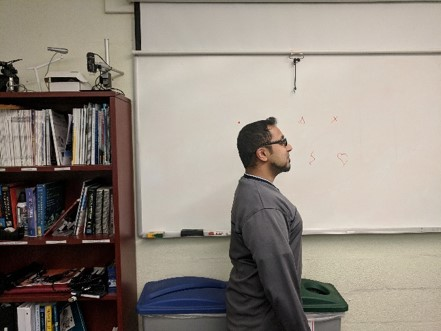
\includegraphics[width=2in]{instruments/melvin1.jpg}
		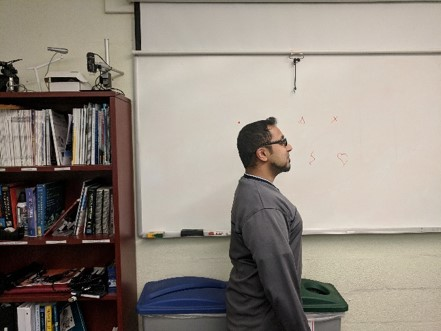
\includegraphics[width=2in]{instruments/melvin1.jpg}
		% 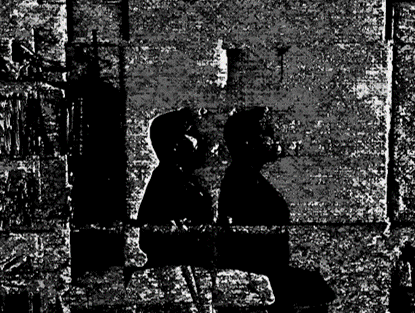
\includegraphics[width=2in]{instruments/melvindisp.png}
		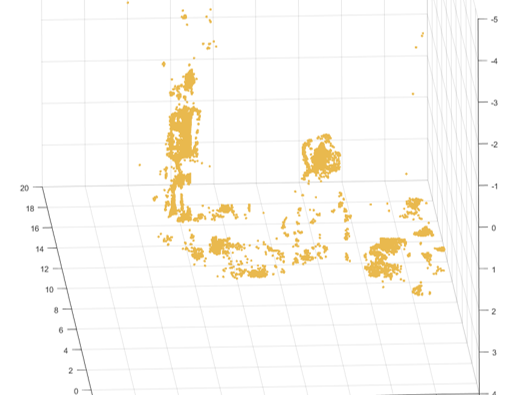
\includegraphics[width=3in]{instruments/melvinSfM.png}
	\caption[Structure from Motion Demonstration]{\centering Demonstration of SfM algorithm conversion of two images to a 3-dimensional point cloud.}
\end{figure}
\cite{RN20}


\subsection{Explicit Methods: LiDAR, Laser Scanning, and Ultrasonic Sensing}
\label{subsec:explicit}
Explicit collection methods are those that directly return a distance value from a sensor. If the scanner itself is non-static, as is the case for laser-scanners and LiDAR devices, the sensor also returns some timestamped orientation parameters to provide a local reference frame.

\subsubsection{LiDAR}
LiDAR scanners vary greatly in accuracy, complexity, and resolution. At the lower end of the spectrum, devices contain one laser and return anywhere from 10-100 points per second along a horizontal plane. The outputs for these LiDAR sensors is timestamped returns of $z$-axis rotation angle $\theta$ and a distance magnitude.

\begin{figure}[!ht]
	\centering
		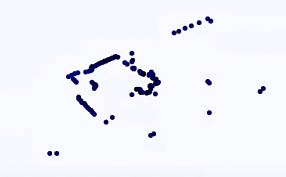
\includegraphics{instruments/crummy_lidar.jpg}
	\caption[Single frame of low tier LiDAR sensor data collection]{\centering Data collected from a single rotation of the [[insert sensor name]] LiDAR device.}
\end{figure}

High end LiDAR devices, such as the HDL-32E used to collect the data in this thesis, have a series of lasers distributed through a range of angles. This allows the LiDAR to provide a much more comprehensive pointset of it's scanned environment. These sensors can provide anywhere between 100,000 and 1.5 million points per second. The typical return for high end sensors is a package of ordered data the return the timestamp of the data, the rotation angle of the sensor, and a vector containing the distance returns of each sensor. Knowing the offset angle of each laser, the dataset can be easily converted into spherical coordinates, and recast in cartesian coordinates. These sensors typically provide a distance uncertainty of $\pm 2 cm$ or lower.

\begin{figure}[!ht]
	\centering
		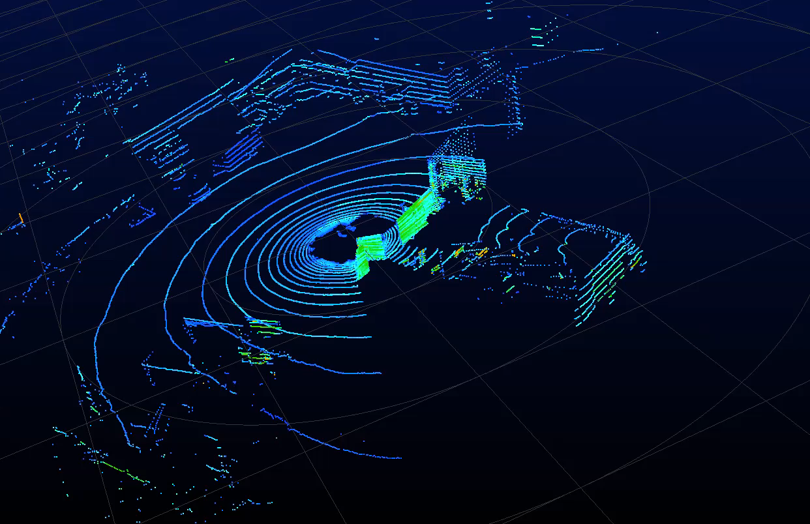
\includegraphics[width=3in]{instruments/HDL-32Esingle.png}
	\caption[Single frame of a high tier LiDAR sensor data collection]{\centering Data collected from a single rotation of the HDL-32E LiDAR device.}
\end{figure}

\subsubsection{Laser Scanning}
[[add]]

\subsubsection{Ultrasonic Sensing}
[[add]]



%%
\section{Sensor Fusion}
\label{sec:fusion}
[[alpha compensator]]
[[particle filter]]
[[kalman filter]]

%%
\section{Point Cloud Pre-processing Methods}
\label{sec:preprocessing}
\subsection{Registration}
\subsubsection{Position Data}
UAVs contain a number of localization measures. Typically implemented are a GPS, an Inertial Measurement Unit, and some form of computer vision. When data from these elements are fused via one of the methods described in the previous section, all six parameters of the global position of the UAV can be accurately obtained (x, y, z, pitch, roll, and yaw).

When onboard position data is collected, concatenating individual collection frames becomes a matter determining the transformation matrix between frames using the orientation and position of the UAV, and applying small corrections based on a combination of RANSAC and Intrinsic Shape Signatures (defined in the next section).


\subsubsection{Intrinsic Shape Signatures}
To stitch individual frames together, distinctive, repeatable features from each frame are found, and the most likely transformation between the frames is calculated via RANSAC estimation. There are numerous ways to classify distinctive features, but the results in this thesis focus on Intrinsic Shape Signatures due to its reliability and computational efficiency.
An intrinsic shape signature consists of two things:

\begin{enumerate}
	\item An intrinsic reference frame.
	\item A highly discriminative feature vector encoding the 3D shape characteristics.
\end{enumerate}

\subparagraph{Intrinsic Reference Frame Calculation}
To calculate the orientation of the Intrinsic Reference Frame, the relationship of a point, $p_{i}$, with the points inside of it's neighborhood is calculated. The neighborhood is described by any points within distance $r_{density}$ to interest point, $p_{i}$.

\begin{enumerate}
	\item Compute a weight for each point $p_{i}$ inversely related to the number of points within 2-norm distance $r_{density}$:
	
		\begin{equation}
		w_{i}=  \frac{1}{||p_{j} \mid |p_{j}-p_{i}| < r_{density}||}
		\end{equation}

		This weight is used to compensate for uneven sampling of the 3D points, so that points at sparsely sampled regions contribute more than points at densely sampled regions. 

	\item Compute a weighted scatter matrix $cov(p_{i})$ for $p_{i}$ using all points $p_{j}$ within distance $r_{frame}$:
	
		\begin{equation}
		cov(p_{i})= \sum{|p_{j}-p_{i}| < r_{frame}}\frac{w_{j}(p_{j}-p_{i})(p_{j}-p_{i})^{T}}{ \sum{|p_{j}-p_{i}| < r_{frame}}w_{j}}
		\end{equation}
		
	\item Compute the covariance matrix eigenvalues in order of decreasing magnitude and their resulting eigenvectors.
	\item $p_{i}$ is now the origin of the intrinsic frame, with $e^{1}$, $e^{2}$, and their cross product as the $x$, $y$, and $z$ axes, respectively \cite{RN60}.
\end{enumerate}

\subparagraph{3D Shape Feature Extraction}
The goal of the extraction is to create a view invariant “feature” vector providing us with some unique qualities about the point relationships within the intrinsic reference frame. At each point in the point cloud, or in increments of voxel stride size s, a sphere of some desired radius r centered at pi is created and divided into 66 distinct partitions in angular space ($\theta, \psi$). A distinctive feature vector with 66 values is then computed by summing the radial distances $\rho_{i}$ in each bin \cite{RN60}.

\begin{figure}[!ht]
	\centering
		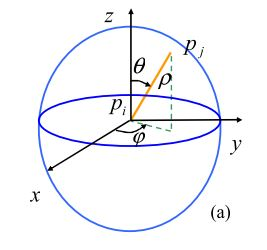
\includegraphics{ISSfeaturevector2.jpg}  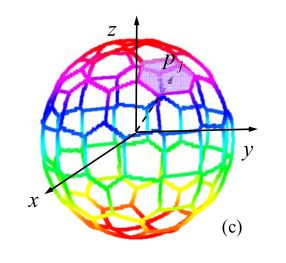
\includegraphics{ISSfeaturevector.jpg}
	\caption[Intrinsic Shape Signature feature vectors]{\centering Feature vector calculation via spherical bin decomposition \cite{RN60}.}
\end{figure}

\subsection{Filtering}
To minimize the amount of noise in the resulting dataset, a statistical approach requiring each point to have k neighbors within d standard deviations from the mean density radius of the cloud. This allows for controlled outlier removal, and a smoother cloud with fewer sharp edges.
\begin{equation}
	P_{x} = p_{i} \mid \sum_{j=1}^n |p_{j} - p_{i}| \leq (r_{density} + d) \geq k
\end{equation}

\begin{figure}[!ht]
	\centering
		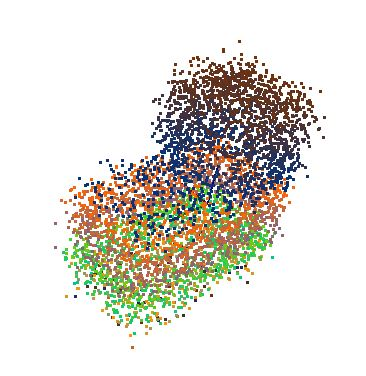
\includegraphics[width=2in]{l_block_pt_cloud10pnoise.jpg} 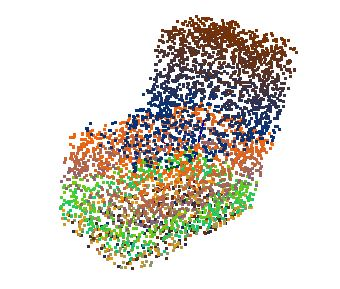
\includegraphics[width=2in]{l_block_pt_cloud10pnoiseFILTEREDk100std05.jpg}
	\caption[Effects of noise filter on simulated point cloud objects]{\centering The effects of noise filtering on a simulated L block with 10\% induced noise.}
\end{figure}


\subsection{Down-Sampling}
Down-sampling is the process of fixing a point cloud’s mean density to a voxel of size n. This is done by iterating the voxel throughout the cloud’s entire volume and replacing all points occupying a voxel with a single point in the mean position of the voxel. For an $n$-dimensional feature-set, the downsampling equation can be defined by Equation~\ref{eq:nddownsample}

\begin{equation}
	\label{eq:nddownsample}
	p_{new} (i) = \frac {\sum_{p(i) \in V}^{N} p(i) }  {N}
\end{equation}

Where $p(i)$ represents the $i^{th}$ point in the dataset, $V$ represents the bounding box of the voxel in $n$-dimensional space, and $N$ represents the total number of points inside the voxel. The result os this equation is the average position of the points inside the voxel.

Figure~\ref{intro:downsampling} shows the results of a simulated shape of initial point-to-point average distance of 0.05 inches downsampled with a voxel size of 0.25 $in^{3}$.

\begin{figure}[!ht]
	\centering
		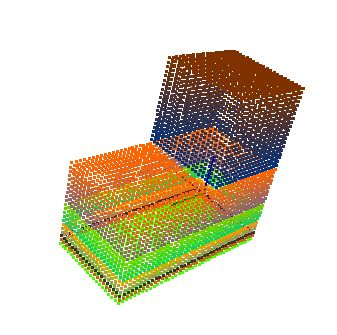
\includegraphics[width=2in]{l_block_pt_cloud} 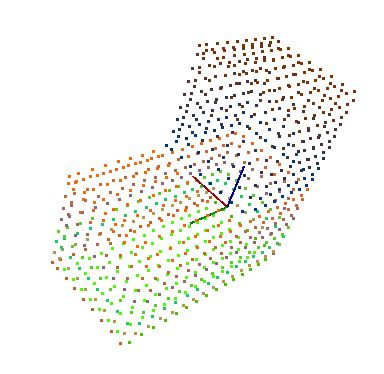
\includegraphics[width=2in]{l_block_pt_cloudDOWNSAMPLE025.jpg}
	\caption[Effects of down-sampling on simulated point cloud objects]{\centering A simulated L block point cloud down-sampled with voxel size = 0.25 $in^{3}$.}
	\label{intro:downsampling}
\end{figure}

Downsampling is crucial for processing poinclouds. The obvious benefit is decreased computation time, but it also allows for us to control the density of the point cloud. Controlling the cloud density allows for meshing parameters to be non-modular, as the input cloud can be forced to a desired density. Section~\ref{subsec:meshing} describes the meshing steps in more detail.

\subsection{Handling Occlusion} 
Occlusion is a common issue in the perception world, defined by the lack of information in an image / 3D scan due to other objects blocking a direct view. A simple example: In 3D scene reconstruction from images, it is impossible to accurately reconstruct the contents inside an opaque box because the images do not provide any information on this space. This is occlusion. In the field, it is nearly impossible to fully avoid occluded datasets when scanning an object via LiDAR equipped UAVs. It is crucial to be able to develop methods to alleviate this problem.

\begin{figure}[!ht]
	\centering
		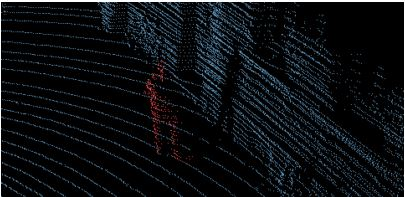
\includegraphics{occluded_man.jpg}
	\caption[Demonstration of occlusion]{\centering Section of a building occluded by an object in the foreground \cite{RN13}.}
\end{figure}

\subsubsection{Range Segementation}
\label{subsubsec:rangeseg}
In urban scanning situations, it is nearly impossible to avoid scan noise. This can come in the form of humans passing by, parked cars, street lights, other buildings, trees, bushes, and a slew of other objects that may come between the scanner and the desired object. Biasuttia et. al. propose a way to cast these interruptions to the surface they desire to map by converting the xyz point cloud to a range image --- a three parameter map of distance $r$ from the device plotted against $\theta$ and $\phi$, the rotation about the $z$ and $x$ axes, respectively.

Once the points are cast to a range image, a range histogram is created. The histogram is segmented into $S$ classes, and the centroid of each class is calculated using the following equation.

\begin{equation}
	C_{s}^{i} = \frac{\sum_{b\in C_{s}^{i}} b  \times h_{s}(b)}{\sum_{b\in C_{s}^{i}}h_{s}(b)}
\end{equation}

Any centroids within some user-defined distance, $\tau$, are merged as a single cloud.

\begin{equation}
	d(C_{s}^{i}, C_{r}^{j}) = |C_{s}^{i} - C_{r}^{j}|
\end{equation}

An algorithm built under the pretext of Gaussian diffusion is then used to project points with a significantly different normals to conform with their range image neighbors. This approach requires structured data that is also time-stamped. In the equation below, $u$ represents the $(\phi, \theta)$ coordinates of a point the merged dataset, and $\Omega$  represents the full range image of the merged dataset, and $\eta$ represents the orthogonal projection of each pixel in the range image. The aim is to solve the following disocclusion problem.

\begin{equation}
		\begin{cases}
			\frac{\partial u}{\partial t} - \Delta u = 0 \in \Omega \times (0,T) \\
			u(0,x) = u_{0}(0) \in \Omega
		\end{cases}
\end{equation}

When scanning large objects, this method proves to be quite effective at removing sources of noise that are significantly smaller than the object being scanned. For buildings, bridges, and large-scale structures, this is a necessary first step in removing excess noise / unnecessary information from the cloud \cite{RN13}.

\subsubsection{Informed Shape Estimation}
\label{subsubsec:informedshape}
Occlusion is the cause of two main problems. The first being the unnecessary information provided by objects blocking the instruments view to the desired target, which is dealt with via the diffusion of objects from the foreground into the background via the range segmentation method show in the previous section. The second --- far more relevant to the approach outlined in this thesis --- is the lack of complete information provided by the sensor. This can be most easily explained by making an analogy to photography. If one takes a picture of the front of a box, there is no possible way to say with certainty what the back of the box looks like. In 3D point processing, the problem is the same. Informed shape estimation attempts to tackle this problem by applying a shape with known parameters to the object point cloud and modifying the shape parameters to minimize the following cost function:

\begin{equation}
	C = \sum_{i=0}^{N}{p(i) - p_{proj}(i)}
\end{equation}

Where $N$ represents the number of points in the set, $p(i)$ represents the $i^{th}$ point in the set, and $p_{proj}(i)$ represents the closest point on the applied shape who's unit normal vector matches within some tolerance, $\tau$.

\begin{equation}
	p_{proj}(i) = arg_{min} \frac{p(i) \bullet l(j)}{||l(j)||} \in p_{normal}(i) \bullet l_{normal}(j) \geq \tau
\end{equation}

\begin{equation}
	\label{eq:newtonraph}
	x_{k+1} = x_{k} - \frac{C(x_{k})}{C'(x_{k})}
\end{equation}

Using a Newton Raphson interative regression, shown in equation \ref{eq:newtonraph} the cross section parameters are modified to minimize the cost required to projection points to the estimated surface. This technique is iterated throughout the long axis of the object, allowing for crucial information such as deformation to be retained. The power in this method is in it's ability to fill information in heavily occluded areas, at the cost of having a narrow scope. Informed shape estimation makes the following assumptions:

\begin{enumerate}
	\item Objection deformation is planar. Calculating the length plane removes the information involving multi-axial deformation.
	\item Cross-section is undamaged thoughout the length of the object. Information regarding damage which alters the objects cross section will be lost when points are projected to the estimated cross section.
	\item The target object can be defined via simple parameters such as length, height, width, and thickness.
\end{enumerate}

\begin{figure}[!ht]
	\centering
		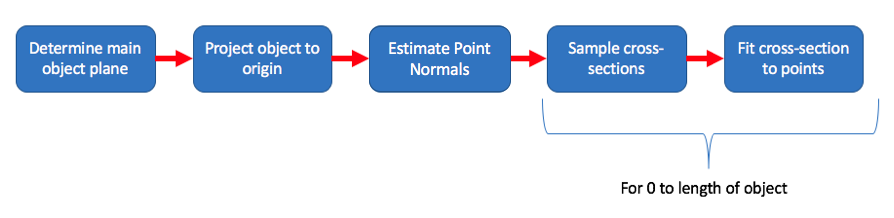
\includegraphics[width=5in]{cross-section-estimation/flowchart.png}
	\caption[Flow chart of informed shape estimation algorithm]{\centering A flowchart of the informed shape estimation algorithm.}
\end{figure}

In many object scanning situations, it is not unreasonable to assume the cross-section of the object is known. Forcing the point cloud to conform to a uniform shape allows for avoidance of heavy amounts of noise.

\begin{figure}[!ht]
	\centering
		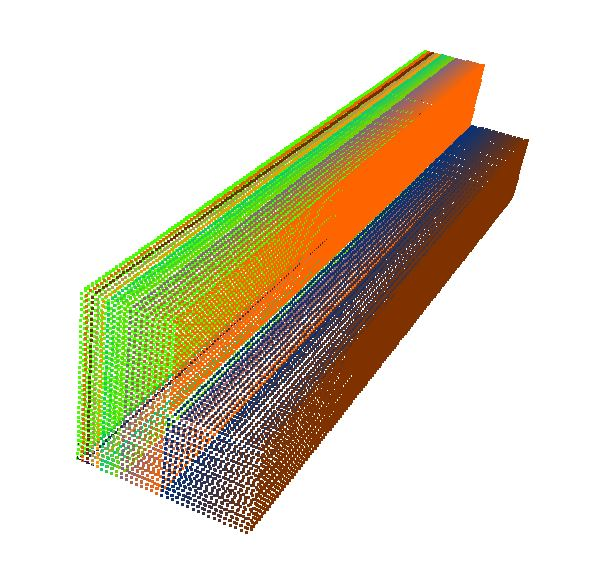
\includegraphics[width=2in]{cross-section-estimation/noiselessbeam(10x10x5).JPG}
		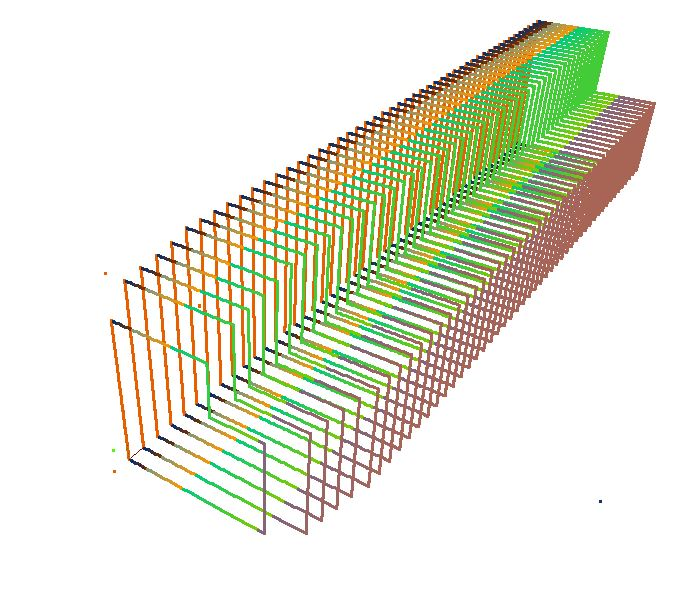
\includegraphics[width=2in]{cross-section-estimation/newtonraphsonconvergence(10x10x5).JPG}
	\caption[Demonstration of the Informed Shape Estimation algorithm on a simulated point cloud.]{\centering Demonstration of the Shape Estimation algorithm on a simulated beam of known dimensions 10x10x5" (left). The iterator converges to dimensions 10.67x10.55x4.87".}
\end{figure}




 


%%
\section{Machine Learning for Object Recognition and Segmentation}
\label{sec:machinelearning}
\subsection{Supervised Methods --- Neural Networks}
\subparagraph{Definitions}
It is difficult to define how a Convolutional Neural Network works without first defining a convolution. To detect distinctive features in a dataset – from a machine’s perspective – the dataset needs to be modified to enunciate those features. Key features in machine vision include edges, corners, and areas with distinctive geometry. Convolutions are the key to bringing these features to the forefront of the image.
A convolution kernel is a weighted square matrix of dimensions m, and depth equaling the rank of the feature space of the dataset. The kernel acts as a filter for the image as it strides from supervoxel to supervoxel. At each step, the dot product of the kernel with data values inside the current super-voxel provide a convolved image of the dataset while retaining characteristic features. The equation below illustrates the math behind a convolution kernel. $C$ represents the convolved image, and $x_{i}$ and $w(i)$ are the $i^{th}$ point and weight of $N$ points located inside the voxel.

\begin{equation}
	C_{new} = \sum_{i}^{N}  w(i) x_{i}
\end{equation}

Another type of convolution is called pooling, or subsampling. This convolution steps through the dataset with a stride value greater than one, resulting in a smaller image of the original set. In pooling, the kernel will pull either the largest intensity from each super-voxel, or the average intensity of the data points inside the super-voxel. This allows for the machine to decrease the size of the dataset while maintaining distinctive features.

\begin{equation}
	C_{new} = \frac{\sum_{i}^{N}  x_{i}}{N}
\end{equation}

\subparagraph{Convolutional Neural Networks}
Convolutional Neural Networks (CNNs) are modeled after the visual cortex in the brain. They consist of layers of convolutional networks. Each network contains “neurons” with simple feature reception fields. Through layers upon layers of these networks, objects can be classified. The biases and weights on these networks can be adjusted based on learning algorithms REF 1 in proposal. CNNs have become the standard in feature classification for image processing, but the accuracy that they provide comes at the price of processing time. 
Every CNN can be broken down into the following steps: Convolution, max/mean pooling, activation function, fully connected layer, repeat. The diagram below illustrates the overarching structure of a basic Convolutional Neural Network:
\begin{figure}[!ht]
	\centering
		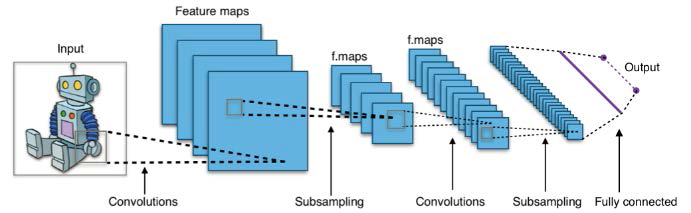
\includegraphics[width=6in]{cnn.png}
	\caption[High level flow chart of a convolutional neural network]{\centering Map of a convolutional neural network with two hidden layers [ref]}
\end{figure}

In the case of point cloud processing, the input is a raw xyz set of some size n x 3. The first step in the network is a series of convolutions of the dataset. Each kernel in the layer contains m x m x 3 trainable weights, which are iteratively modified using a steepest descent numerical solver during the training phase of the system. The convolved images are stacked in a block, called a feature map, or convolutional layer. From there, the convolved images are pooled (or subsampled) to condense the size of the image stack. 
At this point, there is a large stack of feature maps draw from the original input dataset. In a simple linear system, these features are combined into a single weighted summation function, where the input is each individual feature value, and the output is a vector representing the probability of the image belonging to a certain class.

\begin{equation}
\begin{bmatrix}
C_{1} \\
\vdots \\
C_{n}
\end{bmatrix}  =  \begin{bmatrix} w_{1,1} & \hdots & w_{1,m+1} \\ \vdots & \ddots & \hdots \\ w_{n,1} & \hdots & w_{n, m+1} \end{bmatrix}  \begin{bmatrix} f_{1} \\ \vdots \\ f_{n} \\ 1 \end{bmatrix}
\end{equation}

The equation above represents the transformation from feature space to the “fully connected layer.” $C_{i}$ represents the probability of the input image belonging to class $i$, and $f_{i}$ represents the value of the ith feature in the feature map. 
Linear classification methods limit the versatility of the CNN, as many object distinctions do not follow a linear pattern in $n$-dimensional space. To account for this, most CNNs – including the ones utilized in this paper – incorporate a de-linearizing element dubbed the “activation function.” The activation function applies a nonlinear operation to the values in the convolution layer, which allows for the CNN to become a very powerful nonlinear fit function. Typical activation functions include the hyperbolic tangent function, the sigmoid function, and – most popularly – the rectifier function. Each of these functions are show in the figure below:

\begin{figure}[!ht]
\centering
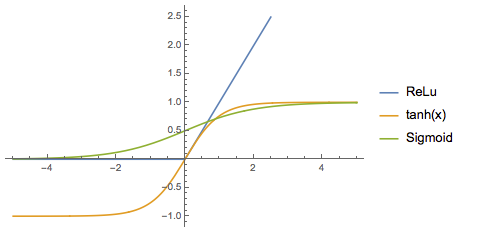
\includegraphics[width=5in]{cnnReLu.png}
\caption[Common CNN non-linear activation functions]{\centering Visualization of commonly used non-linear activation functions}
\end{figure}

From input to output, all CNNs have the same skeleton structure, with a varying number of layers between the raw input and the fully connected layer:

\begin{figure}[!ht]
	\centering
		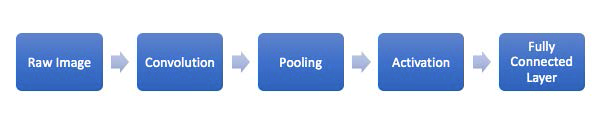
\includegraphics[width=6in]{cnn_flow.png} 
	\caption[Block diagram of CNN flow]{\centering Block diagram of a CNN$'$s skeleton structure}
\end{figure}

For the system to be accurate, the weights for each convolution and connection must be trained. This training is done through a process called backpropagation. An image-set of known classifications is fed to the untrained system, and the error between the system’s classification and the true classification of each image is used to update the weights iteratively until the machine’s class prediction closely resembles ground truth. Most algorithms use numerical solving methods to sharply diminish the number of iterations required for convergence. The “gradient descent” method is commonly used in the machine learning world due to its rapid convergence properties and low computational complexity. The method is shown below:

\begin{equation}
	x_{k+1} = x_{k} - \gamma \nabla F(x_{k})
\end{equation}

$F(x)$ is described as the residual function. It is the diference between the result of the cost function $C(x)$, and the current $x$ variable values.

\begin{equation}
 F(x) =
\begin{bmatrix}
C_{1} \\
\vdots \\
C_{n}
\end{bmatrix}  -  \begin{bmatrix} w_{1,1} & \hdots & w_{1,m+1} \\ \vdots & \ddots & \hdots \\ w_{n,1} & \hdots & w_{n, m+1} \end{bmatrix}  \begin{bmatrix} f_{1} \\ \vdots \\ f_{n} \\ 1 \end{bmatrix} 
\end{equation}

The speed, accuracy, and versatility of a CNN are functions of the number of hidden layers, the size of the convolutional layers, the type of activation functions, and the size and versatility of the training dataset \cite{RN7}. Because CNNs -- and all supervised learning methods -- require a large amount of training data, they do not fit within the scope of the proof of concept inside of this paper. However, supervised learning has proven to be one of the most effective forms of classification, and will be addressed in the future work section of this thesis.

\subsection{Unsupervised Methods}

\subsubsection{K-means Clustering}
K-means clustering is an iterative method that groups $n$-dimensional datasets into $k$ clusters based on a minimization of the Euclidean distance cost function $|x-c|^{2}$. Initially, $k$ centroids are placed randomly inside the dataset, and all data points are placed in bins $S$ depending on which centroid minimizes their cost function. At each iteration, the cluster centroids $c_{i}$ are re-calculated. Criteria for convergence is a maximum Euclidean distance change $\sigma$ between centroid position $c_{n}$ and $c_{n+1}$.
\begin{equation}
	arg min_{S} \sum{i=1}^{k} \sum{x \in S_{i}} |x - c_{i}|^{2}
\end{equation}

K-means clustering is arguably the most well known clustering method, and is useful for a massive variety of naïve classification problems. In any situation where the bin-size is known and the data is clearly separated in some feature space $\mathbb{R}^{n}$, k-means proves to be an effective clustering method. It's ease of implementation comes at the cost of computate. As with most unsupervised clustering methods, the major downside to k-means is it's non-reusability. Where supervised methods require their computational time upfront during the training phase, k-means requires significant computational time with every dataset. It does not develop a set of multiplier weights, so it must start the clustering algorithm from scratch with each new input set.

\subsubsection{Fuzzy C-means Clustering}

Fuzzy C-means (FCM) is very similar to K-means clustering. Once again, points are iteratively grouped to k centroids based on their Euclidean distance to the centroid. The significant difference is that points do not belong exclusively to a single group. Instead, points are weighted by their degree of belonging in each cluster.

\begin{equation}
	c_{k} = \frac{\sum{x}w_{k}(x)^{m}x}{\sum{x}w_{k}(x)^{m}}
\end{equation}

Each point is provided a weight vector w [0, 1] for its likelihood of belonging in each cluster, where the weight function is as follows:

\begin{equation}
	w_{ij} = \frac{1}{\sum_{k=1}^{c}(\frac{|x_{i}-c_{j}|}{|x_{i}-c_{k}|})^{\frac{2}{m-1}}}
\end{equation}

Fuzzy clustering is differentiated from k-means in that points are not isolated to a singular cluster until the final thresholding step after FCM has reached it's exit criteria. This allows for all points in the dataset to continually effect the location of every cluster centroid. FCM finds it's worth in $n$-dimensional datasets that are not clearly segregated by their cost functions, but do have a series of denser clouds. FCM is even more computationally intensive than it's counterpart, k-means, because it must iteratively calculate the location of every point in relationship to every centroid, and then also calculate the weights of each point in reference to each centroid.

\subsubsection{Aggomerative and Dvisive Hierarchical Clustering}
In Agglomerative clustering, each point is initially considered its own cluster. Iteratively, the points are grouped together based on a user-defined cost function – in this case, Euclidean distance. The exit conditions for this method are either convergence upon a set of clusters, or a predefined number of clusters.
Divisive clustering approaches the clustering problem in an exactly opposite fashion. The algorithm initializes the dataset as a single cluster and iteratively splits the remaining clusters until reaching the same exit conditions as the Agglomerative method.


\begin{figure}[!ht]
\centering
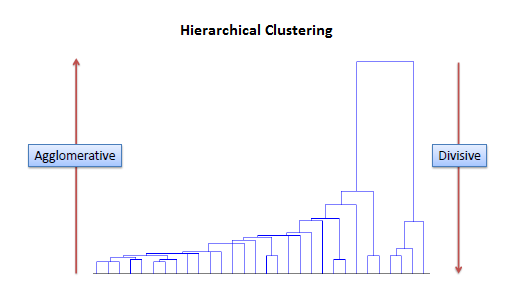
\includegraphics[width=4in]{divisiveAgglomerative.png}
\caption[Comparison of divisive and agglomerative clustering methods]{Comparison of divisive and agglomerative hierarchical clustering}
\end{figure}

Hierarchical clustering is not as computationally efficient as k-means or FCM, as the number of calculations it must make for each point is drastically higher. At each iteration, each point, $p_{i}$, is compared with every point inside of it's bin, to determine what bin it will be divided into. This means Hierarchical clustering methods occupy $\mathcal{O}(n^{3})$ time complexity space, and requires $\mathcal{O}(n^{2})$ memory. This makes Hierarchical clustering very unwieldy with medium and large datasets. However, it proves to be one of the more robust supervised segmentation algorithms, as the cost function is easily modifiable by the user.


\subsubsection{Euclidean Distance Clustering}
Perhaps the simplest of the algorithms listed above, Euclidean distance clustering operates on the pretense that objects are separated significantly enough spatially from another that clustering points based on their proximity to other points in the cloud is sufficient to properly segment the dataset. This algorithm involves no iterative process, and requires three inputs: Maximum point-to-point distance, $r$, minimum number of points per cluster, $k_{min}$, and maximum number of points per cluster, $k_{max}$.

Euclidean clustering occupies the lowest time complexity and memory space of it's unsupervised brethren, and does not require an expected bin-size.

\subsubsection{Comparison of Methods}

 \begin{table}[!ht]
     \centering
           \caption[Comparison of Unsupervised clustering methods]{\centering Comparision of unsupervised clustering methods on various simulated point clouds}
     \begin{tabular}{ | c | c | c | c | c | }
     \hline
      K-means & Fuzzy C-means & Agglomerative & Divisive & Euclidean \\ 
      \hline
      		\includegraphics[width=2cm]{2d-cluster-tests/k-means/concentric.jpg}
      & 
      		\includegraphics[trim={0 1cm 0 1cm},clip, width=2cm]{2d-cluster-tests/fcm/concentric.jpg}
      & 
      		\includegraphics[width=2cm]{2d-cluster-tests/agglomerative/concentric.jpg}
      &

      &
      		\includegraphics[width=2cm]{2d-cluster-tests/euclidean-distance/concentric.jpg}
      \\ \hline
      
            \includegraphics[width=1.5cm]{2d-cluster-tests/k-means/lines.jpg}
      & 
             \includegraphics[trim={0 1cm 0 0.5cm},clip,width=1.9cm]{2d-cluster-tests/fcm/lines.jpg}    
      & 
             \includegraphics[trim={0 1cm 0 0cm},clip,width=1.5cm]{2d-cluster-tests/agglomerative/lines.jpg}    
      &

      &
             \includegraphics[trim={0 1cm 0 1cm},clip, width=1.5cm]{2d-cluster-tests/euclidean-distance/lines.jpg}    
      \\ \hline
      
           \includegraphics[trim={0 1cm 0 1cm},clip,width=1.5cm]{2d-cluster-tests/k-means/blob.jpg}
      & 
           \includegraphics[trim={0 0cm 0 0cm},clip,width=1.5cm]{2d-cluster-tests/fcm/blob.jpg} 
      & 
           \includegraphics[trim={0 1cm 0 1cm},clip,width=1.5cm]{2d-cluster-tests/agglomerative/blob.jpg} 
      &

      &
           \includegraphics[trim={0 0.5cm 0 0.25cm},clip,width=1.5cm]{2d-cluster-tests/euclidean-distance/blob.jpg} 
      \\ \hline
      
            \includegraphics[width=1.5cm]{2d-cluster-tests/k-means/solid_circles.jpg}
      & 
            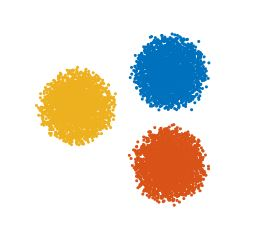
\includegraphics[width=1.5cm]{2d-cluster-tests/fcm/circles.jpg}
      & 
            \includegraphics[width=1.5cm]{2d-cluster-tests/agglomerative/solid_circles.jpg}
      &

      &
            \includegraphics[width=1.5cm]{2d-cluster-tests/euclidean-distance/solid_circles.jpg}
      \\ \hline
      
            \includegraphics[width=1.5cm]{2d-cluster-tests/k-means/plane.jpg}
      & 
            \includegraphics[trim={0 0cm 0 0.25cm},clip,width=1.75cm]{2d-cluster-tests/fcm/plane.jpg}
      & 
            \includegraphics[width=1.5cm]{2d-cluster-tests/agglomerative/plane.jpg}
      &
      
      &
            \includegraphics[width=1.5cm]{2d-cluster-tests/euclidean-distance/plane.jpg}
      \\ \hline
      
      \end{tabular}
      \end{table}


\section{Converting a Discrete Point Cloud to a Bounded Area Surface Mesh}
\label{subsec:meshing}
\subsubsection{Definition of a Surface Mesh}
\label{subsubsec:surfdef}
Surface meshes, in simple terms, are a series of connected areas defined by their vertices in $n$-dimensional space. The areas are typically triangles or tetrahedrons, and form together to define a continuous surface area using discrete data points. There are many ways to store surface mesh objects, but they all require two components:

\begin{enumerate}
	\item A set of vertices, $v$, occupying $n$-dimensional space $\mathbb{R}^{n}$.
	\item A set of connection indices $I$, which dictate how the vertices connect to one another.
\end{enumerate}

In a fully bounded surface mesh, the combination of each triangulation object creates a shell, which represents the surface area of the shape.

\begin{figure}[!ht]
	\centering
	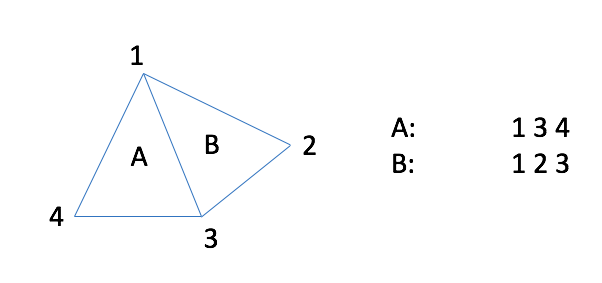
\includegraphics[width=3in]{points2surface/surface_mesh.png}
	\caption[Simple example of surface mesh components]{Visualization of necessary components in a surface mesh.}
	\label{meshing:surface_mesh}
\end{figure}

Typical file-types for surface meshes contain the location of the vertices in 3-dimensional space, followed by definitions for their connectivity in index form.

\subsubsection{Definition of a Volume Mesh}
A volume mesh is defined with the same parameters as a surface mesh, with the key difference being that it defines the entire exterior and interior of the object.
One application --- and the target application for this thesis --- is finite element analysis, a numerical method for solving structural analysis problems through discretization of individual elements in an $n$-dimensional geometry and calculating their relative parameters in reference to their connected neighbors.

\subsubsection{Definition of a Boundary Representation (B-REP)}
Boundary Representations, often called the ''skin'' of a solid object, consist of two parts: topology and geometry. The topological portion is made from the faces and vertices created by a surface mesh. In the boundary representation of an object, the edges bounding a triangulation object -- or face -- is defined as a loop. The geometric portion consists of equations defining the edges and faces. There are a number of different ways in which the geometry of an object's surface area can be modeled, but the most common is the Non-Uniform Rational Basis Spline (NURBS).

\begin{figure}[!ht]
	\centering
		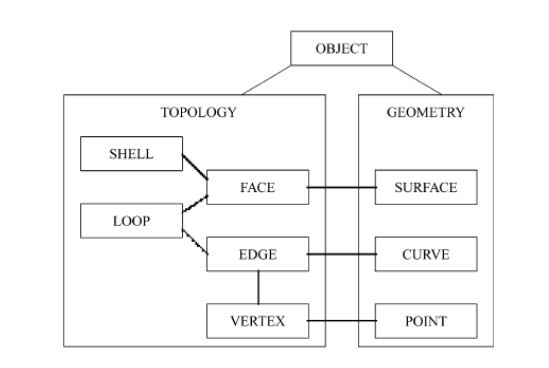
\includegraphics[width=3in]{cadTypes/brep.jpg}
	\caption[Components of a boundary representation.]{\centering An overview of the components involved in a boundary representation of a solid object \cite{Stroud2006}.}
\end{figure}

\subsubsection{Non-Uniform Rational Basis Spline (NURBS)}
NURBS curves are a method of interpolating a discrete set of vertex points into a continous function. Each vertex point is considered a ``control point,'' and a series of smooth polynomials are concatenated locally over individual sets of control points. An $n$-dimensional NURBS curve $f(u)$ can be defined ast the following:

\begin{equation}
	f(u) = \frac    {   \sum_{i=0}^{K-1} w_{i} B_{i,n}(u) P_{i} }
				 	{  \sum_{i=0}^{K-1} w_{i} B_{i,n}(u) }
	\label{nurbs:weightedbspline}
 \end{equation}
 
 Where $P_{i}$ represents the $i^{th}$ control point, $n$ represents the polynomial degree of the blending function, $B_{i,d}(u)$, and $w_{i}$ represents the weight of the $i^{th}$ control point. The equation is simplified accordingly by inserting the rational basis function relationship described in Equation~\ref{nurbs:rationalbasis} to the piecewise B-Spline equation shown in Equation~\ref{nurbs:weightedbspline}.
 
\begin{equation}
	R_{i}(u) = \frac    {   w_{i} B_{i,n}(u)}
				 		{  \sum_{i=0}^{K-1} w_{i} B_{i,n}(u) }
	\label{nurbs:rationalbasis}
 \end{equation}
 
 Leaving us with the following relationship:
 
 \begin{equation}
 	f(u) = \sum_{i=0}^{K-1} R_{i,d}(u) P_{i}
\end{equation}

Using these weighted concatenations, smooth surfaces are generated from a series of sharp geometric edges.


\begin{figure}[!ht]
	\centering
		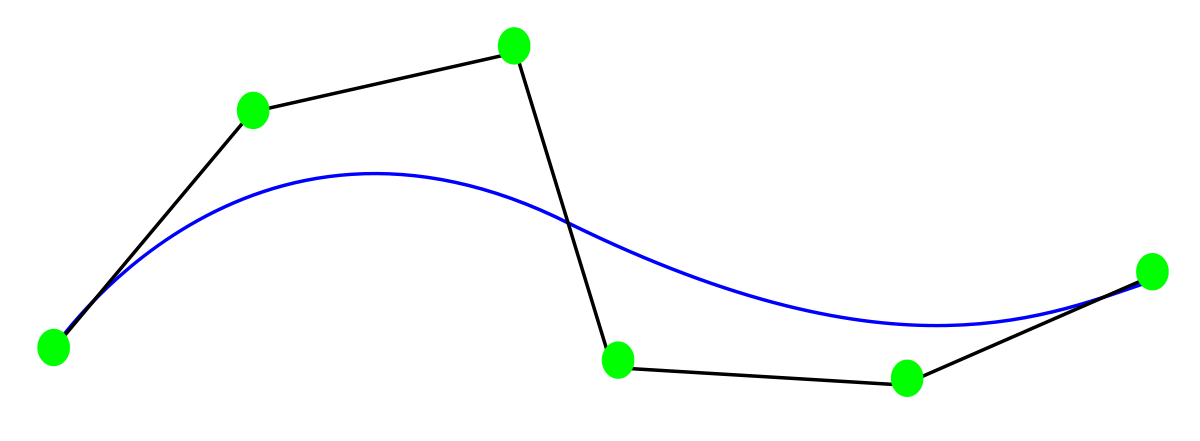
\includegraphics[width=2in]{cadTypes/nurbs.png}
	\caption[Example of a 2-dimensional nurbs spline.]{\centering A 2-dimensional example of a nurbs spline. Green points represent the control points, $P$, black lines represent their connectivity, and the blue line represents one possible nurbs spline.}
\end{figure}


\subsubsection{Delaunay Triangulation}
\label{subsubsec:delaunay}
Surface meshing is the method of inferring a continuous shape topology from a discrete, $n$-dimensional point cloud. There are many different approaches to converting from discrete points to surface meshes, but at their core, nearly all of them rely on the Delaunay triangulation method.
Delaunay triangulation finds its routes in Voronoi tessellation, a method of constructing non-overlapping geometrical tiles. Voronoi tessellation states the following:
For a given set of points in space, $\{P_{k}\}$ --- $k$ = 1, \ldots, $K$, the regions \{$V_{k}$\} are polygons assigned to each seed point $P_{k}$, such that $V_{k}$ represents the space closer to $P_{k}$ than any other point in the set.

\begin{equation}
	V_{k} = \{P_{i} \mid |p - P_{i}| < |p - P_{j}|, \forall j \neq i \}
\end{equation}

If every point pair sharing a Voronoi boundary are connected, the result is a triangulation object encasing the pointset. This object is referred to as a Delaunay triangulation \cite{RN65}.

\begin{figure}[!ht]
\centering
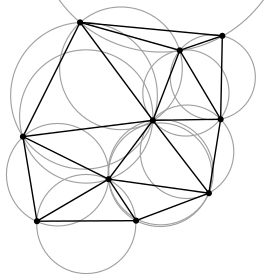
\includegraphics{delaunay.png}
\caption[2D delaunay triangulation]{\centering Visual represention of a 2-dimensional delaunay triangulation process}
\end{figure}

\subsubsection{Advancing Front / Marching Triangles}
The Advancing Front method is common in computer graphics software – especially in procedurally generated games – because of it’s speed and computational simplicity.

In the Advancing Front method, a mesh is constructed by progressively adding tetrahedra starting at the boundaries of the previous surface elements. At each iteration, the mesh boundary is propagated further across the set of surface points. New tetrahedra are determined based on the minimal delaunay triangluation between the boundary vertices and unreferenced points in space. Each new triangulation object is created by adding a single unreferenced point at a time \cite{RN66}.

\subsubsection{Scale Space Reconstruction Method}
At a grand scale, the Scale Space Reconstruction Method aims to optimize surface meshing in the face of discrete point cloud data. No matter how accurate or dense a point cloud may be, there is no way to verify the topology defined by the cloud is accurate to the true object topology. To simplify this ill-posed problem, and reduce mesh quality damage due to noisy points, the Scale Space algorithm casts the raw point cloud to a space of scale N by iteratively calculating the mean curvature of a neighborhood of points and casting each point pk to it’s nearest point on the curve. This results in a far more uniform point cloud, which can mesh via Delaunay triangulation at a high quality level. Once the meshing has occurred, the pointset is then recast to its original scale to maintain complex features. 

\textbf{Algorithm 1:} Mean Curvature Calculation

	\textbf{Input:} A point set $P$, a query point $p$, and a radius $r$.
	
	\textbf{Output:} A point $p'$, the result of one discrete step of the mean curvature calculation applied to $p$.
\begin{lstlisting}[escapeinside={(*}{*)}]
	for ( (*$p$*) in (*$P$*) )
		get (*$neighbors$*) from (*$p$*)
		if num(neighbors) < 5
			remove (*$p$*)
		set (*$p_{bar} = \frac{\sum_{q \in neighbors} w(q)q}{\sum_{q \in neighbors}w(q)}$*)
		set (*$C = \sum_{q \in neighbors} w(q)(q-p_{bar})(q-p_{bar})^{2}$*)
		set (*$v_{0} = arg_{min} eigenvector(C)$*)
		set (*$p' = p - \langle p - p_{bar}, v_{0} \rangle v_{0}$*)
		(*$p' \cdot n = \frac{p-p'}{|p-p'|} \cdot sign(\langle p - p', p \cdot n \rangle ) $*	
\end{lstlisting}

\textbf{Algorithm 2:} Scale Space Iterator

	\textbf{Input:} A point set $P$, a number of iterations $N$, and a radius $r$
	
	\textbf{Output:} A modified point set $P_{N}$


\begin{lstlisting}[escapeinside={(*}{*)}]
	for (*$p$*) in (*$P$*)
		set (*$p.origin = p$*)
	set idx = 0
	for ( i = 0, \ldots, N-1 )
		new_idx = mod(idx, 2) + 1
		for (*$p \in P_{idx}$*)
			(*$p' = MCC(p, P_{idx}, r)$*)
			store (*$p'$*) in (*$ P_{new_idx}$*)
			(*$p'.origin = p.origin $*)
		if ( idx > 0 )
			remove (*$P_{idx}$*)
		idx = new_idx
\end{lstlisting}

Using the Ball Pivoting Algorithm \cite{ballpivot}, a reconstruction is implemented that does not change the location of the smoothed vertex positions or add new vertex positions. In a nutshell, the Ball Pivoting Algorithm iterates a sphere of radius $r$ thoughout the pointcloud. If three points are located on the sphere, a triangulation with those vertices is created. If no points are found, the radius is expanded.

At this point, the vertices of the smoothed mesh are recast to zero-scale ( their initial points in the point cloud). The result is a mesh built based on a smoothed input, with minimual noise reduction in the process \cite{RN67}.

\begin{table}[h]
\centering
\caption[Effect of increasing scale in a scale space reconstruction]{Effect of increasing scale in a scale space reconstruction}
\begin{tabular}{ | c | c | c | }
\hline
& 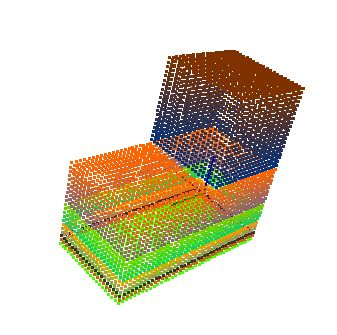
\includegraphics[width=3cm]{l_block_pt_cloud.jpg}
	Clean Point Cloud
& 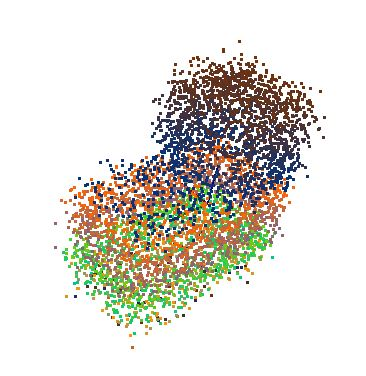
\includegraphics[width=3cm]{l_block_pt_cloud10pnoise.jpg}
	10\% Induced Noise
\\
\hline
Scale Space 3 & 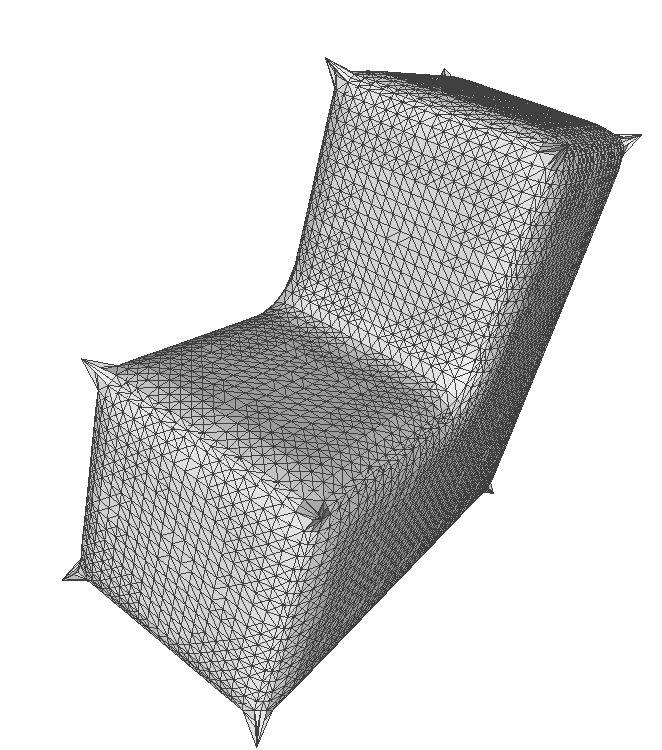
\includegraphics[width=3cm]{scalespace/clean/scalespace3.png} & 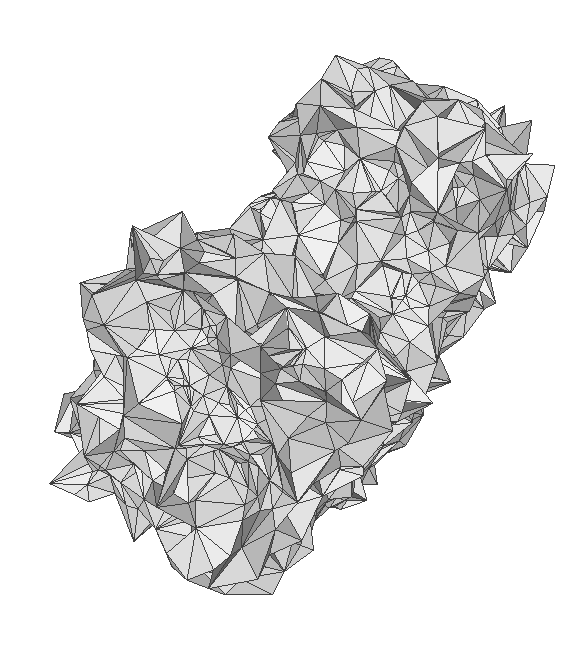
\includegraphics[width=3cm]{scalespace/10pnoise/scale3.png}
\\
\hline
Scale Space 5 & 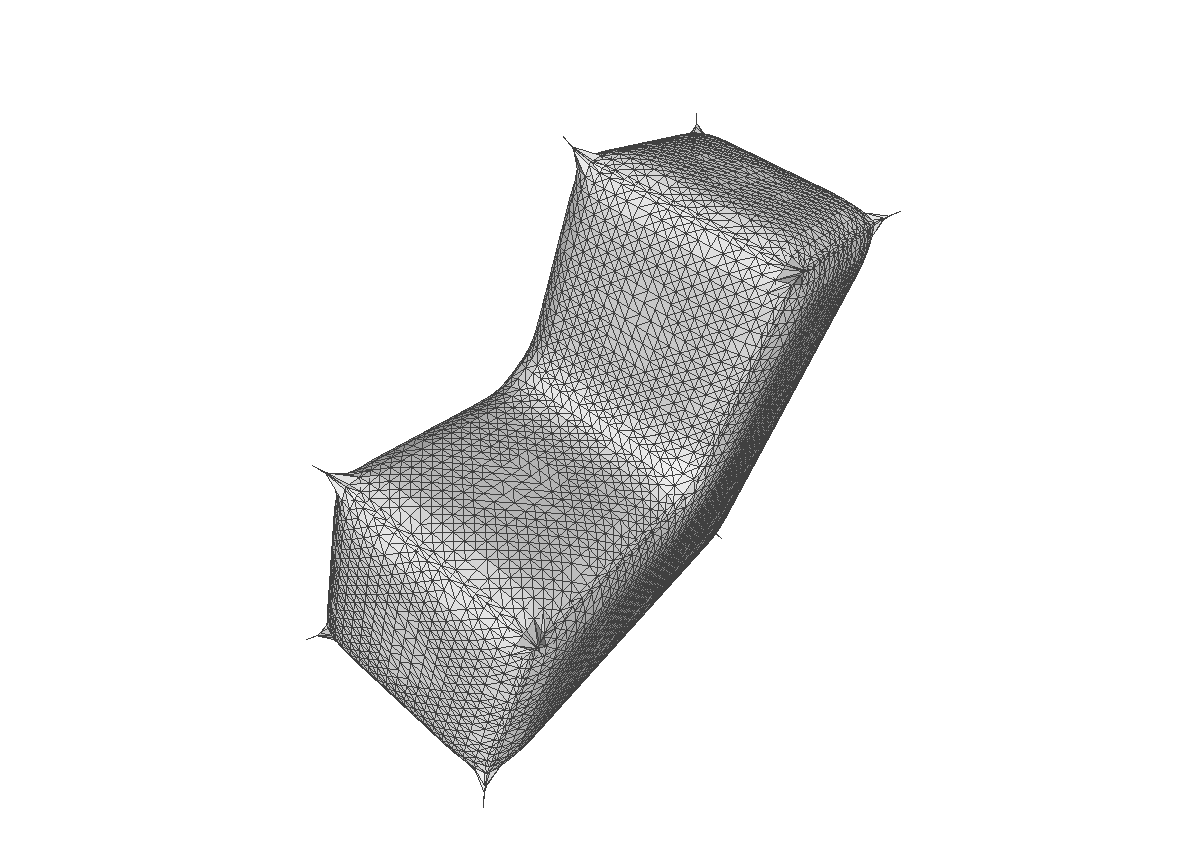
\includegraphics[width=3cm]{scalespace/clean/scalespace5.png} & 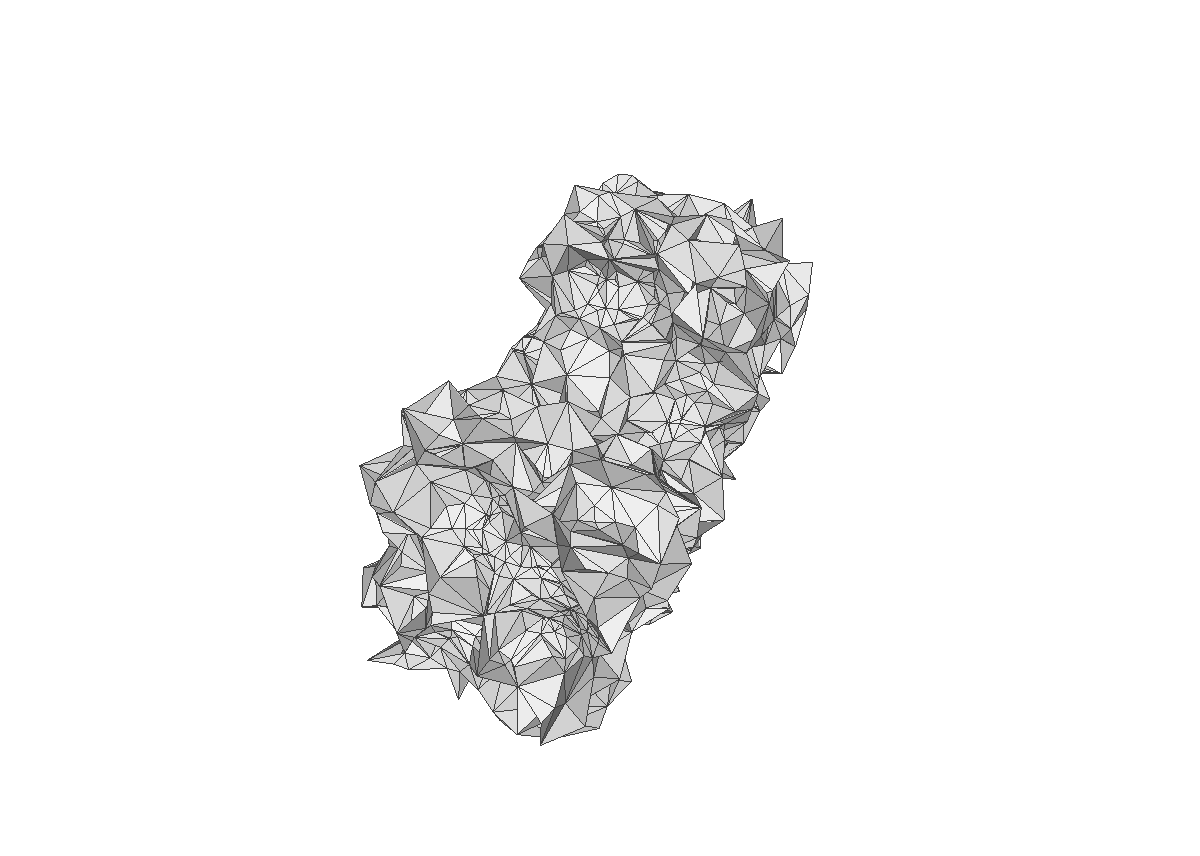
\includegraphics[width=3cm]{scalespace/10pnoise/scale5.png}
\\
\hline
Scale Space 10 & \includegraphics[width=3cm]{scalespace/clean/scalespace10.png} & \includegraphics[width=3cm]{scalespace/10pnoise/scale10.png}
\\
\hline
\end{tabular}
\end{table}

\subsubsection{Hole Patching, Fairing, and Refinement}

Surface meshes, defined in Section~\ref{subsubsec:surfdef}, contain vertices and faces. Inherently, they do not contain any methods to maintain a bounded volume. For this reason, it is necessary to detect discontinuities in the mesh, and develop a method to resolve them. Two types of mesh edges are defined in this section: A full edge, and a half edge.
A full edge occurs when an edge is referenced by more than one polyhedral object. What this means in physical terms is that the edge is not on the boundary of the shape. Half edges, on the other hand, are only referenced by a single polyhedral object. Half edges are indicators of holes in the mesh, as they are unreferenced anywhere else in the surface area.

\begin{figure}[!ht]
	\centering
		\includegraphics[width=3in]{edgevshalfedge.png}
		\caption[Example of an edge vs. a half edge]{\centering A visualization of the difference between an edge and a half edge. Half edges are outlined in blue.}
\end{figure}

To remedy this, a delaunay triangulation search is run between half edges, and create the least costly triangulations. While this seals the mesh, the result is a non-uniform surface mesh, where the new sections have a far larger surface area than the surrounding mesh. For this reason, refinement is necessary to return the mesh to an isotropic state.

[[REFINEMENT]]

\subsection{Mesh Optimization}
\label{subsec:meshoptimization}
Now that the objects in the cloud are properly segmented, they must be meshed in a way that is both accurate to the real-world definition of the object and suitable to be converted from a surface mesh to a volumetric mesh.

\subsubsection{Criteria for Mesh Quality and Failure Criteria for Volumetric Conversion}

\subparagraph{Failure Criteria}
The first criterion for surface mesh compatibility with volumetric conversion is “water-tightness.” Meaning, there are no gaps, holes, or unbounded edges in the triangulation. These gaps can be quantified as any edge in a polyhedron that is referenced by no other polyhedron in the triangulation.
The other criteria are more abstract in nature and are more difficult to detect and handle independently. These criteria are defined as mesh “Quality.” Quality is a quantification of the level of simplicity of a triangulation object by evaluating ratios of different elements in the triangulation.

\begin{figure}[!ht]
	\centering
		\includegraphics[width=2in]{triangulation_definitions.JPG}
		\includegraphics[width=3in]{bad_tetrahedra.JPG}
		\caption[Definitions for triangulation quality measures]
		{\centering Definitions for triangulation quality measures, and typical shapes with poor quality. $R$ = circumsphere radius, $r$ = inscribed sphere radius, $l$ = edge length.}
		\label{fig:meshquality}
\end{figure}

It is easy to categorize meshes by quality via visual inspection, but in order to resolve low quality areas autonomously, what it means to be "low quality" must be explicitly defined mathematically. Table~\ref{table:meshquality} lists some of the ratios to define a mesh's quality level. Low  quality  values  in  mesh  return  problematic  polyhedrons  for  volumetric  conversion,  typically  looking  like  those  shown  in  figure \ref{fig:meshquality}.

\begin{table}[!ht]
	\centering
		\caption{Quantification of mesh quality}
		\begin{tabular}{| c | c |}
			\hline
			Inner/outer radius edge ratios & $Q_{1} = \frac{l_{min}}{R}$, $Q_{2} = \frac{r}{l_{min}}$
			\\ \hline
			Aspect ratio & $Q_{3} = \frac{r}{R}$
			\\ \hline
			Edge ratio & $Q_{4} = \frac{l_{min}}{l_{max}}$
			\\ \hline
			Volume ratio & $Q_{5} = \frac{V}{l_{max}^{3}}$
			\\ \hline
		\end{tabular}
		\label{table:meshquality}
\end{table}


\subsubsection{Voronoi Relaxation / Lloyd's Algorithm}
\label{optimization:voronoirelaxation}
\begin{figure}[!ht]
	\centering
		\includegraphics[width=4in]{voronoirelaxation.PNG}
		\caption[Demonstration of voronoi relaxation over several iterations]
		{\centering From right to left: Voronoi relaxation over 1 iteration, 5 iterations, 10 iterations, and 15 iterations}
		\label{fig:voronoirelaxation}
\end{figure}

Voronoi  relaxation  operates  on  the  same  principle  as  k-means  clustering.  At  each  iteration,  the  centroid  of  each  Voronoi  region  is  calculated,  and  the  concurrent  vertex  is  moved  to  the  centroidal  location.  At  convergence,  the  resulting  mesh  is  uniform  in  tetrahedron/triangulation  size.  Voronoi  relaxation  can  modify  a  shape’s  topology  significant  due  to  its  heavy  smoothing  capabilities  \cite{RN61}.

\subsubsection{Optimal Delaunay Triangulation}
Delaunay triangulation, as described in Section~\ref{subsubsec:delaunay}, optimizes the connectivity for a finite point set through voronoi propagation. To calculate the optimal triangulation of the pointset defined by a discrete set of vertices, the vertices are unfixed from their intial points in space. As a caveat, because this optimization method involves shift the locations of the vertices, the topology of the mesh is altered in the process.

To define an optimal triangulation, given a continuous convex function $f$ on $\Omega$ and $1 \leq p \leq \inf$, and triangulation $\tau^{\ast} \in P_{N}$  the following criteria is used:

\begin{equation}
	Q ( \tau^{\ast}  , f, p) = \substack{inf \\ _{\tau \in P_{N}} } (\tau , f, p)
\end{equation}

[[ what does this mean / what does it mean to be optimal ]]

\subsubsection{Mesh Perturbation}
While  Voronoi  relaxation  and  ODT  are  large  scale  smoothing  and  refinement  techniques,  they  have  no  constraints  on  slivers  present  in  the  mesh.  Perturbation  and  exudation  are  are  necessary  to  oust  any  slivers  remaining  in  the  triangulation.  Slivers  are  defined  as  any  triangulation  with  an  angle  less  than  $\alpha$,  a  user-defined  parameter.  The  algorithm  iteratively  increases  the  angles  created  in  a  triangulation  by  applying  a  pseudo-random  perturbation  vector,  $p_{v}$,  to  vertices  coincident  with  triangulations  defined  as  slivers.  If  the  perturbation  results  in  a  success,  resulting  triangulation  is  kept.  Otherwise,  a  new  perturbation  vector  is  calculated  to  create  a  higher  quality  triangulation  \cite{RN63}. 

\subsubsection{Mesh Exudation}
Exudation  again  is  a  method  to  remove  any  slivers  remaining  in  the  surface.  Each  point  in  a  tetrahedron  classified  as  a  sliver  is  assigned  a  weight  based  on  its distance  relationship  to  it’s  neighbors.  The  point  weighted  most  heavily,  then,  is  the  tip  of  the  sliver,  and  is  modified  to  place  the  tetrahedron  within  the  acceptable  bounds  of  mesh  quality  \cite{RN64}. 












%%%%%%%%%%%%%%%%%%%%%%%%%%%%%%%%
% Chapter: 		Hypothesis
\chapter{Objective, Hypothesis, and Technical Approach}
\label{chap:purposestatement}

\section{Research Objective}
The objective of this thesis is to develop and validate a software pipeline capable of segmenting point cloud data of some expected density $\rho$ and within some accuracy tolerance $\sigma$ into clusters of meaningful shapes, and convert the resulting clusters into surface meshes valid for conversion to simply connected volumes. The research described in this thesis is inarguably very wide in application and scope, but is geared specifically towards Structural Health Monitoring and Non-Destructive Test and Analysis. The results of this Master's thesis are a proving ground for rapid scanning, meshing, and analysis of real-world objects.

\section{Hypothesis Statement}
The claims made in this thesis are the following:

\begin{enumerate}
	\item Point cloud scans oriented towards a specific object can be segmented to isolate said object with or without supervised clustering methods.
	\item Provided a point cloud meets some required criteria, there is a generalized algorithm to convert raw clouds to volumetrically adaptable surface meshes.
\end{enumerate}

The second hypothesis attempts to nail down an explicit definition of what it means for a mesh to be volumetrically compatible. Determining what conditions a point cloud must meet to be properly meshed, and what modifications can be made and to what extent are all problems that have yet to be fleshed out completely in the domain of real world to simulation conversion technology. This thesis aims to quantify criteria for raw point clouds to be meshed properly, criteria for smoothing limits before the resulting volume can no longer be realistically considered to have similar properties to it's real world counterpart, and criteria for a surface mesh to be successful converted to a volume. 

Knowing these limits allows for collection of point cloud data for the sake of information extraction to be much more educated. Defining criteria for the amount of a surface that must be visible in the cloud, accuracy limits, and smoothing limits are critical for creating an automated approach to finite element analysis on real objects with reliable results. The following chapters quantify the effect of parameter modification at each step of the algorithm.

While this thesis does not provide vetted parameters for assured volume compatibility, there is significant exploration into what parameters work and what cause a mesh to fail. Interestingly enough, a mesh that is aesthetically pleasing is demonstrated to be a successfully convertible mesh.

\section{Technical Approach}
To fully evaluate the effect of each step in the algorithm and test the robustness of the proposed algorithm, it is applied to a series point clouds, both simulated and real, with varying levels of noise and occlusion. The goal is to accurately mimic the cloud resolution of the test device, and to proof the robustness of the algorithm at resolutions expected from other measurement devices. Simulated data has been crafted to model resolution, accuracy, and occlusion levels with the approaches that follow:

\subsection{General: Zero Noise}
The pipeline is first explored with a fabricated point cloud of varying resolutions. This point-cloud does not omit any features of the simulated room to mimic occlusion, and has zero simulated noise. In short, every point in the cloud is in its true position in 3-dimensional space. These clouds shown below are optimal cases and are entirely unacquirable with any instruments in use today, or in the forseeable future. They do, however, serve as a proof of concept for the meshing pipeline as a form of optimal results.

\begin{figure}[!ht]
	\centering
	\includegraphics[width=3in]{simulated-lab-scan/full_noiseless_cloud.png}
	\caption[Simulated high density lab point cloud ]{\centering Virtual lab point cloud with zero induced noise and occlusion. there are 114,808 points in the cloud.}
	\label{sim:noiselessdense}
\end{figure}

\subsection{General: Estimated Noise and Occlusion}
As the instruments within the scope of this thesis vary in expense, acquireability, and technical specifications, it is necessary to simulate their expected results. This can be done by modeling each instrument's acquisition technique, and applying that technique to the simulated room point cloud at a high density. The following figure set outline the collection methods of each technique, and their simulated accuracy.

\begin{figure}[!ht]
	\centering
	% [[\includegraphics[width=3in]{2 percent noise cloud}]]
	\caption[Simulated high density lab point cloud with 2cm noise induction]{\centering Simulated high density lab point cloud with 2 centimeter noise induction.}
	\label{sim:2cmdense}
\end{figure}


\subsection{LiDAR: Velodyne HDL-32E}
The Velodyne HDL-32E is a high end LiDAR device capable of collecting 700,000 points per second at a frame rate of 20 Hz (rotations per second). It is equipped with 32 lasers aligned from +\ang{10.67} to -\ang{30.67}

As described in Section~\ref{subsec:explicit} of the introduction, LiDAR devices provide explicit distance feedback in spherical coordinates, where each point is defined by $\phi$, its angle about the $z$-axis, $\theta$, its angle about the $y$-axis, and $r$, the absolute distance from the sensor. The return can be classified as ordered data, and easily mimicked in simulation by creating a series of solid objects, simulating the output of the LiDAR, and simulating the LiDAR motion. This allows for fast simulation of point cloud collection with varying levels of noise, occlusion, and sample rate.

To simulate noise in the LiDAR scans, it is a simple matter of adding the measured uncertainty to distance metrics collected by the simulated sensor. It should be noted that to reduce computation time, no continuous surfaces are created, and the simulation relies on nearest cross product distances of points in the cloud to determine the sensor data return. An unfortunate artifact of this method is the inability to guarantee correct occlusion effects, as simulated rays can be cast through a continuous object created by a discrete pointset of non-infinite density. Figure~\ref{lidarsim:100psample} shows the collection capabilities of the HDL-32E at 100\% sampling rate. There are 73,175 point inside the cloud.

\begin{figure}[!ht]
	\centering
	\includegraphics[width=3in]{simulated-lab-scan/lidarSim/100psample.png}
	\caption[Simulated LiDAR scan at 100\% sampling rate]{\centering Simulated LiDAR scan of the virtual lab point cloud at 100\% sampling rate. The red trail shows the collection path of the sensor.}
	\label{lidarsim:100psample}
\end{figure}

In the test run in this thesis, only one in every five LiDAR scan frames are used in the post-processing steps. The true LiDAR scan data is therefor reduced to 20\% of the original sample set. This is mainly due to redundancy and unwieldy cloud sizes (700,000 points per second becomes unruly in a very short period of time). Figure~\ref{lidarsim:20psample} shows the result of the simulation at 20\% sampling rate. There are 18,973 points in the cloud shown below. It is likely the true scan data will contain many more points before being downsampled due to redundant point collection. The algorithm built here does not include the same target point more than once.

\begin{figure}[!ht]
	\centering
	\includegraphics[width=3in]{simulated-lab-scan/lidarSim/20psample.png}
	\caption[Simulated LiDAR scan at 20\% sampling rate]{\centering Simulated LiDAR scan of the virtual lab point cloud at 20\% sampling rate. The red trail shows the collection path of the sensor.}
	\label{lidarsim:20psample}
\end{figure}

The LiDAR is fixed to a mobile table of fixed height during the collection process. This means the amount of acquireable data on the beam's shape is severely limited. In Section~\ref{results:realscan}, the effects of this scanning technique can be seen in the lack of thickness data on the horizontal portion of the beam.

\begin{figure}[!ht]
	\centering
		\includegraphics[width=2in]{cloudCollection/velodyneLiDAR.jpg}
		\caption[Velodyne LiDAR Operation]{\centering Visualization of how to the Velodyne HDL-32E operates.}
\end{figure}

Figure~\ref{technical:lidarcompare} shows a comparison between a single frame of simulated HDL-32E LiDAR data and a true scan with the device. The simulation proves to be quite similar in results to the true scans, which will prove to be useful for future endeavors beyond this one.

\begin{figure}[!ht]
	\centering
		\includegraphics[width=2in]{cloudCollection/lidar5frames.png}
		% \includegraphics[width=2in]{cloudCollection/lidarSimulatedCollection.JPG}
		%[[add a decent simulated collection figure]]

	\caption[Comparison of simulated and real HDL-32E scan data]{\centering Comparison of simulated and real HDL-32E scan data.}
	\label{technical:lidarcompare}
\end{figure}

The individual scans are iteratively concatenated in the manner described in Figure~\ref{technical:lidarcompare}. At each iteration, a new frame is loaded, and the Intrinsic Shape Signature map for the cloud is generated. Using a RANSAC fitting algorithm, the transformation between the newest frame and the previous frame is calculated, and added to the global transformation matrix. The new frame is transformed and added to the global cloud. This technique allows for comparison of only two frames at a time, instead of having to calculation the Intrinsic Shape Signature map of the concatenated point cloud, which increases in size at each iteration.

\begin{figure}[!ht]
	\centering
		%flow chart of cloud concatenation process
	\caption[Flow chart of point cloud concatenation process.]{\centering Flow chart of point cloud concatenation process.}
	\label{technical:lidarcompare}
\end{figure}

\subsection{Stereogrammetry and Photogrammetry}
Stereogrammetry and Photogrammetry are both highly dependent on the camera quality, speed of motion, and feature density of the image. As these methods depend on matching descriptive features between images, the resulting cloud is typically far more sparse than what would be obtained with a LiDAR device.


\subsection{Segmentation Method Exploration}

To mesh a point cloud object properly, the object must be isolated robustly from the point cloud. This section deals with the discovery of the most effective and robust methods for segmentation of unordered point cloud into meaningful clusters in an entirely automated way.

As a result, the methods evaluated in this thesis are reserved purely to those which are classified as unsupervised. Selected based on potential success, popularity, and ease of implementation, the following segmentation methods are analyzed in Chapter~\ref{chap:results}: K-Means Clustering, Fuzzy C-Means Clustering, Euclidean Distance Clustering, and Agglomerative Hierarchical Clustering.
\end{enumerate}

Detailed descriptions of how these algorithms operate, as well as general use cases and a list of pros and cons, can be found in Section~\ref{sec:machinelearning}. Each method is applied to the simulated datasets, and their results are visualized. Based on observation, an optimal clustering method is found and the resulting segments are run through the meshing and optimization phase of the algorithm.

\subsection{Initial Mesh Exploration}

There are two algorithms for the initial mesh construction intended for evaluation in this thesis: Scale Space Reconstruction and Avancing Front. Advancing front provides no robustness to noise or occlusion in the dataset, but guarantees no overlapping faces, so could be viable with the addition of hole patching and the optimization stage. Scale Space Reconstruction, on the other hand, is designed specifically for handling noisey, variable density datasets. It does not prevent overlapping elements, so removal of these elements must be added to the pipeline for this case. It should also be noted that because of Scale Space Reconstruction's casting steps (described in Section~\ref{subsec:meshing}), it is far more computationally expensive than the Advancing Front method.

These methods are evaluated on their abilities to create comprehensive surface areas and their quality metrics after hole patching and refinement.

\subsection{Optimization Steps}

The goal of the optimization process is to remedy or remove any elements in the mesh that violate the criteria for volumetric conversion compatibility. These criteria are defined in Section~\ref{subsec:meshoptimization}. Each step in the optimization pipeline specializes in modifying specific characteristics of the mesh which can be defined as having low quality using the metrics in Section~\ref{subsec:meshoptimization}.

The first step in the optimization process is Lloyd Optimization, or Voronoi Relaxation. LLoyd optimization seeks to resolve triangulations with low [[add quality metrics resolved by lloyd optimization]]. Lloyd Optimization comes with the caveat that it moves the location of the shape vertices, so this step comes at the cost of modifying the topology collected directly by the sensor. Depending on the accuracy of the collection instrument, this can be either a curse or a blessing.

The next step is the Optimized Delaunay Triangulation method. ODT is another relaxation method capable of modifying the object's topology in order to increase the overall quality of the mesh. Between Lloyd Optimization and ODT, every quality metric should -- while not guaranteed to be so -- be within the tolerance set by the exit conditions applied, with the exception of slivers. To remedy these, perturbation and exudation are necessary.

Perturbation and exudation are included in the pipeline of algorithm for two reasons. The first being that both Lloyd Optimization and ODT are quality improving algorithms for all of the parameters listed in Section~\ref{subsec:meshoptimization}, except for slivers. Perturbation and Exudation both specialize in the removal of these tetrahedra. The second reason is to relieve the effects ODT often has on the mesh. ODT can have a ``pock-marking'' effect upon the mesh, as it optimizes using delaunay radii as a cost function, and this often means vertices are shifted towards the interior of the surface mesh. 
 

\subsection{Final Mesh Verification}

The final verification of the meshes output by the algorith occurs in two stages. The first being a measure of each desired quality parameter to assure the mesh meets the criteria set in this paper. The second is an exportation of the mesh to AutoDesk Fusion, which has in-built functionality to convert surface meshes to boundary representations and bounded volumes. If both of these verifications are successful, the resulting mesh is placed under typical loading conditions to compare it's response to the expected response of the true object.












%%%%%%%%%%%%%%%%%%%%%%%%%%%%%%%%%
%Chapter			Results
\chapter{Results}
\label{chap:results}
\section{Simulated Data: Zero Noise}
The first instance of the algorithm is the control set, and first step in the ground-up development of the pipeline. There is no noise induced in the system, and all objects are significantly separated in 3-dimensional space. Figure~\ref{zeronoise:raw} shows the point cloud. The total number of points in the cloud is [[insert number of points]], average point to point distance is [[insert point to point distance]], and beam point-to-point distance is [[insert beam point to point distance]]. Beam dimensions are 3.048m (10ft) with a cross-section of the following specifications:


\begin{centering}
Width: 12.7cm (5in)
\\Height: 12.7cm (5in)
\\Thickness: 0.635cm (0.25in) \\
\end{centering}

Figure~\ref{zeronoise:raw} shows the unmodified pointcloud at high resolution. The dataset in this section has zero noise and zero occlusion, and provides insight into what each step of the mesh optimization process accomplishes. Including the ground plane, there are 17 distinct objects in this point cloud.


\begin{figure}[!ht]
		\centering
		\includegraphics[width=3in]{simulated-lab-scan/0noise/sim-lab-0noise.jpg}
		\caption[Simulated laboratory point cloud data with zero noise induced]{\centering Simulated laboratory point cloud data with zero noise induced.}
	\label{zeronoise:raw}
\end{figure}


While not necessary in the zero noise case, filtering and downsampling prove to be crucial portions of the algorithm. In Figure~\ref{zeronoise:filtered} a filter is applied to remove any points with fewer than 15 neighbors, where neighbors are defined as being within one standard deviation plus the average point-to-point distance of the entire cloud. After filtering, the cloud is subsampled to have a maximum density of 0.1 centimeters squared.


\begin{figure}[!ht]
	\centering
		\includegraphics[width=3in]{simulated-lab-scan/0noise/sim-lab-0noise-DS01-k15std1.jpg}
		\caption[Zero noise simulated data after being filtered with voxel size of 0.1 $in^{3}$, 15 minimum point neighbors at a distance of 1 standard deviation from the mean point to point distance]{\centering Zero noise simulated data after being filtered with voxel size of $0.1 in^{3}$, 15 minimum point neighbors at a distance of 1 standard deviation from the mean point to point distance.}
	\label{zeronoise:filtered}
\end{figure}

The resulting cloud size is [[insert cloud size]], with an average point-to-point distance of 0.1 inches. Being able to actively control the point cloud density is crucial to have control over proper meshing parameters and fail conditions.

\subsection{Segmentation Method Comparison}

With the exception of euclidean distance clustering, each unsupervised clustering method requires a number of bins. For FCM and k-means, these bins represent the centroids of the clusters, and for Hierarchical, they represent the exit condition for number of divisions. Ideally, the number of bins should match the number of desired segmentations, so the bin size is set to 17. Euclidean clustering requires a minimum radius between points as an input. As the mean point-to-point distance is forced to 0.1 inches, a higher value encapsulates surface gaps which are encountered in the non-ideal cases. Setting the distance to 0.5 inches proves to have satisfactory results.

\begin{figure}[!ht]
	\label{zeronoise:segcompare}
	\centering
		\includegraphics[width=3in]{simulated-lab-scan/0noise/all_methods.jpg}
		\caption[Comparison of unsupervised segmentation techniques on a simulated dataset.]{\centering Resulting cloud cluster from a) k-means, 17 centroid b) Fuzzy c-means, 17 centroids c) Agglomerative clustering, 17 bins and d) Euclidean clustering with radius of 0.5 in and a maximum cluster size of 50,000 points.}
	\label{zeronoise:compare}
\end{figure}

It is clear from the results in Figure~\ref{zeronoise:compare} that Euclidean clustering far outshines it's unsupervised brethren in ability to segment the noiseless point cloud in a meaningful way. To clear out undesired segments, criteria on the minimum and maximum cloudsize are imposed. In Figure~\ref{zeronoise:optimal} a minimum cloud size of 3,000 points, and a maximum size of 50,000 is imposed on the segmentation results.

\begin{figure}[!ht]
	\centering
		\includegraphics[width=3in]{simulated-lab-scan/0noise/euclidean-d05max50000min3000.jpg}
		\caption[Euclidean distance segmentation with ideal parameters.]{\centering  Euclidean clustering with radius of 0.5 in, minimum cluster size of 3,000 points and a maximum cluster size of 50,000 points.}
	\label{zeronoise:optimal}
\end{figure}

The filtering and segmentation parameters derived from this zero noise situation are adequate for isolating the beam from the rest of the point cloud.


\subsection{Initial Meshing Methods}
In a zero noise situation, the advancing front method returns a nearly perfect mesh, with the exception of a poor quality polygon linking the rear segment of the mesh. This is caused by the ``marching triangles'' attempting to close the final corners of the mesh. This meshing method provides high quality meshes while maintaining accurate features in zero noise situations, but with the introduction of noise the Advancing Front method quickly fails to produce a reliable initial mesh for successful optimization.

\begin{figure}[!ht]
	
	\centering
		\includegraphics[width=2in]{simulated-lab-scan/0noise/clean/advancingfront.png}
		\includegraphics[width=2in]{simulated-lab-scan/0noise/clean/advancingfront01.png}
		\includegraphics[width=2in]{simulated-lab-scan/0noise/clean/advancingfront02.png}
		\caption[Initial meshing using a raw advancing front approach]{\centering  Result of initial meshing using the advancing front method.}
		\label{zeronoise:advancingfront}
\end{figure}

Figure~\ref{zeronoise:scalespace2} shows the effects of Scale Space reconstruction at scale $S = 2$. The predominantly visible effect is the change in topology of the beam. because of the localized fnunction estimation that occurs during the scale-space casting phase, the planar surface of the beam is reconstructed with a parabolic shape. The overall thickness is reduced.

\begin{figure}[!ht]
	\centering
		\includegraphics[width=2in]{simulated-lab-scan/0noise/clean/scale200.png}
		\includegraphics[width=2in]{simulated-lab-scan/0noise/clean/scalespace201.png}
		\includegraphics[width=2in]{simulated-lab-scan/0noise/clean/scalespace202.png}
		\caption[Initial meshing using a scale space reconstruction with $S = 2$]{\centering  Result of initial meshing using the scale space reconstruction method with $S = 2$.}
	\label{zeronoise:scalespace2}
\end{figure}

As the beam is cast into higher and higher scale-spaces, the thickness of the beam is continually reduced. At scale-space 4 and higher -- shown in Figures~\ref{zeronoise:scalespace4} and \ref{zeronoise:scalespace15}, the beam thickness (originally $\frac{1}{4}$in) is reduced to zero. This is due again to the piecewise function estimation that occurs in the specified scale space. Once all of the points are cast down far enough, they are no longer registered as being in two separate neighborhoods, and are instead identified as belonging to the same 2-dimensional curve.

\begin{figure}[!ht]
	\centering
		\includegraphics[width=2in]{simulated-lab-scan/0noise/clean/scalespace400.png}
		\includegraphics[width=2in]{simulated-lab-scan/0noise/clean/scalespace401.png}
		\includegraphics[width=2in]{simulated-lab-scan/0noise/clean/scalespace402.png}
		\caption[Initial meshing using a scale space reconstruction with $S = 4$]{\centering  Result of initial meshing using the scale space reconstruction method with $S = 4$.}
		\label{zeronoise:scalespace4}
\end{figure}

Figure~\ref{zeronoise:scalespace15} shows the extremes of what the scale space reconstruction can do to alter the topology of a mesh. Because the points are cast to such a high scale, there is virtually no thickness between points on one side of the beam and points on the other. For this reason, the shape is cast as a 2-dimensional object. It is clear that casting an object like the beam to as high a scale as shown here is not viable for initial meshing. 

\begin{figure}[!ht]
	\centering
		\includegraphics[width=2in]{simulated-lab-scan/0noise/clean/scalespace1500.png}
		\includegraphics[width=2in]{simulated-lab-scan/0noise/clean/scalespace1501.png}
		\includegraphics[width=2in]{simulated-lab-scan/0noise/clean/scalespace1502.png}
		\caption[Initial meshing using a scale space reconstruction with $S = 15$]{\centering  Result of initial meshing using the scale space reconstruction method with $S = 15$.}
		\label{zeronoise:scalespace15}
\end{figure}

In the zero noise case, Advancing Front reconstruction proves to be the most accurate to the beam's dimensions. However, as seen in future sections, this method is not robust to noise. Both of these statements are unsurprising, as this reconstruction method does not modify the topology defined by the pointset provided, and therefor directly represents the shape defined by the input cloud.

\subsection{Optimization}
\subsubsection{Effects of Voronoi Relaxation}

Voronoi relaxation, defined in Section~\ref{optimization:voronoirelaxation}, aims to regulate the tetrahedral areas in the mesh by iteratively shifting point vertices to their respective voronoi centroids. This method is effective in increasing the mesh quality ratios defined in Table~\ref{table:meshquality}, with the exception of volume ratio, which can be visualized as slivers in the mesh (Figure~\ref{fig:meshquality}).

The relaxed mesh after 200 iterations of voronoi relaxation is shown in Figure~\ref{zeronoise:advancedlloyd}. Note the uniformity in tetrahedral area, as well as the change topology around the edges of the beam.

\begin{figure}[!ht]
	\centering
		\includegraphics[width=2in]{simulated-lab-scan/0noise/optimized/advancedfrontlloyd00.png}
		\includegraphics[width=3in]{simulated-lab-scan/0noise/optimized/advancedfrontlloyd01.png}
		\includegraphics[width=2in]{simulated-lab-scan/0noise/optimized/advancedfrontlloyd02.png}
		\includegraphics[width=2in]{simulated-lab-scan/0noise/optimized/advancedfrontlloyd03.png}
		\caption[Advancing Front mesh after 200 iterations of voronoi relaxation]{\centering  Result of Advancing Front mesh after 200 iterations of voronoi relaxation.}
	\label{zeronoise:advancedlloyd}
\end{figure}

Voronoi Relaxation has interesting effects of the scale space meshes. The mesh in Figure~\ref{zeronoise:scalespace2lloyd} is a relatively smooth, pock-marked version of the initial scale-space mesh. Notice on the left-most corner of the beam there are a few tall, narrow shapes. These shapes are the slivers remaining in the mesh. The next steps in the optimization process aim to remove these slivers.

\begin{figure}[!ht]
	
	\centering
		\includegraphics[width=2in]{simulated-lab-scan/0noise/optimized/scalespace2lloyd00.png}
		\includegraphics[width=3in]{simulated-lab-scan/0noise/optimized/scalespace2lloyd01.png}
		\includegraphics[width=2in]{simulated-lab-scan/0noise/optimized/scalespace2lloyd02.png}
		\includegraphics[width=2in]{simulated-lab-scan/0noise/optimized/scalespace2lloyd03.png}
		\caption[Scale space reconstruction $S = 2$ after 200 iterations of voronoi relaxation]{\centering Scale space reconstruction $S = 2$ after 200 iterations of voronoi relaxation.}
	\label{zeronoise:scalespace2lloyd}
\end{figure}

Similar results are shown in Figure~\ref{zeronoise:scalespace4lloyd}. This mesh is 2-dimensional due to the scale-space casting, but still shows the effects of voronoi relaxation quite vividly.

\begin{figure}[!ht]
	\centering
		\includegraphics[width=2in]{simulated-lab-scan/0noise/optimized/scalespace4lloyd00.png}
		\includegraphics[width=3in]{simulated-lab-scan/0noise/optimized/scalespace4lloyd01.png}
		\includegraphics[width=2in]{simulated-lab-scan/0noise/optimized/scalespace4lloyd02.png}
		\includegraphics[width=3in]{simulated-lab-scan/0noise/optimized/scalespace4lloyd03.png}
		\caption[Scale space reconstruction $S = 4$ after 200 iterations of voronoi relaxation]{\centering Scale space reconstruction $S = 4$ after 200 iterations of voronoi relaxation.}
	\label{zeronoise:scalespace4lloyd}
\end{figure}


\subsubsection{Effects of Delaunay Optimization}

Delaunay optimization seeks to find the minimal triangulation conditions for the mesh by iteratively shifting the vertices of the mesh to positions that minimize the cost function defined in Section~\ref{subsec:meshoptimization}. For this reason, ``pock-marks'' begin to appear in the mesh, as these positions minimize the Delaunay radii apparent in the mesh. Correcting this phenomenon is a large portion of the reason perturbation and exudation exist in meshing pipeline.

\begin{figure}[!ht]
	\centering
		\includegraphics[width=2in]{simulated-lab-scan/0noise/optimized/advancedfrontlloydodt00.png}
		\includegraphics[width=3in]{simulated-lab-scan/0noise/optimized/advancedfrontlloydodt01.png}
		\includegraphics[width=2in]{simulated-lab-scan/0noise/optimized/advancedfrontlloydodt02.png}
		\includegraphics[width=2in]{simulated-lab-scan/0noise/optimized/advancedfrontlloydodt03.png}
		\caption[Advancing Front mesh after ODT with a 30 second clock cap]{\centering  Result of Advancing Front mesh after ODT with a 30 second clock cap.}
	\label{zeronoise:advancedodt}
\end{figure}

The negative effects of ODT are increasingly apparent at each greater scale of the scale space reconstruction. Any imperfections in the mesh are enunciated by a heavy, vacuum-like extrusion.

\begin{figure}[!ht]
	\centering
		\includegraphics[width=2in]{simulated-lab-scan/0noise/optimized/scalespace2odt00.png}
		\includegraphics[width=3in]{simulated-lab-scan/0noise/optimized/scalespace2odt01.png}
		\includegraphics[width=2in]{simulated-lab-scan/0noise/optimized/scalespace2odt02.png}
		\includegraphics[width=2in]{simulated-lab-scan/0noise/optimized/scalespace2odt03.png}
		\caption[Scale space reconstruction $S = 2$ after ODT with a 30 second clock cap]{\centering Scale space reconstruction $S = 2$ after ODT with a 30 second clock cap.}
	\label{zeronoise:scalespace2odt}
\end{figure}

It is clear at this point that for low thickness objects in zero noise situations, $4^{th}$ scale space is too high, as it results in a zero volume surface mesh. There are no remedies for a mesh that fails to generate any surface hull at all.

\begin{figure}[!ht]
	\centering
		\includegraphics[width=2in]{simulated-lab-scan/0noise/optimized/scalespace4odt00.png}
		\includegraphics[width=3in]{simulated-lab-scan/0noise/optimized/scalespace4odt01.png}
		\includegraphics[width=2in]{simulated-lab-scan/0noise/optimized/scalespace4odt02.png}
		\includegraphics[width=3in]{simulated-lab-scan/0noise/optimized/scalespace4odt03.png}
		\caption[Scale space reconstruction $S = 4$ after ODT with a 30 second clock cap]{\centering Scale space reconstruction $S = 4$ after ODT with a 30 second clock cap.}
	\label{zeronoise:scalespace4odt}
\end{figure}

\subsubsection{Effects of Mesh Perturbation}

Perturbation serves two purposes: To relax any remaining slivers in the mesh (slivers defined in Section~\ref{subsec:meshoptimization}) into higher quality tetrahedra, and to relieve inward deviations created by the ODT step.

In Figure~\ref{zeronoise:advancedperturb}, the result of the Advancing Front mesh after being perturbed for 30 seconds is seen. In this case, there were not many -- if any at all -- tetrahedra that met the criteria to be slivers. The only sliver correct visible is in the lower lefthand corner of the beam. In earlier steps of the algorithm, there is a slight dog-ear, which is now far less exaggerated.

\begin{figure}[!ht]
	\centering
		\includegraphics[width=2in]{simulated-lab-scan/0noise/optimized/advancedfrontlloydodtperturb00.png}
		\includegraphics[width=3in]{simulated-lab-scan/0noise/optimized/advancedfrontlloydodtperturb01.png}
		\includegraphics[width=2in]{simulated-lab-scan/0noise/optimized/advancedfrontlloydodtperturb02.png}
		\includegraphics[width=2in]{simulated-lab-scan/0noise/optimized/advancedfrontlloydodtperturb03.png}
		\caption[Advancing Front mesh after perturbation with a 30 second clock cap]{\centering  Result of Advancing Front mesh after perturbation with a 30 second clock cap.}
	\label{zeronoise:advancedperturb}
\end{figure}

The next figure is the reconstruction at scale space $2$. Again the mesh is severely pock-marked, but far less so than it's predecessor. Provided a higher clock limit, these pock-marks are slightly more relieved, but unfortunately perturbation does not converge at the ``smoothest'' mesh, but at the mesh that satisfies it's constraints for quality.

\begin{figure}[!ht]
	
	\centering
		\includegraphics[width=2in]{simulated-lab-scan/0noise/optimized/scalespace2perturb00.png}
		\includegraphics[width=3in]{simulated-lab-scan/0noise/optimized/scalespace2perturb01.png}
		\includegraphics[width=2in]{simulated-lab-scan/0noise/optimized/scalespace2perturb02.png}
		\includegraphics[width=2in]{simulated-lab-scan/0noise/optimized/scalespace2perturb03.png}
		\caption[Scale space reconstruction $S = 2$ after perturbation with a 30 second clock cap]{\centering Scale space reconstruction $S = 2$ after perturbation with a 30 second clock cap.}
	\label{zeronoise:scalespace2perturb}
\end{figure}



% \begin{figure}[!ht]
% 	\centering
% 		\includegraphics[width=2in]{simulated-lab-scan/0noise/optimized/scalespace4perturb00.png}
% 		\includegraphics[width=3in]{simulated-lab-scan/0noise/optimized/scalespace4perturb01.png}
% 		% \includegraphics[width=2in]{simulated-lab-scan/0noise/optimized/scalespace4perturb02.png}
% 		% \includegraphics[width=3in]{simulated-lab-scan/0noise/optimized/scalespace4perturb03.png}
% 		\caption[Scale space reconstruction $S = 4$ after perturbation with a 30 second clock cap]{\centering Scale space reconstruction $S = 4$ after perturbation with a 30 second clock cap.}
% 	\label{zeronoise:scalespace4perturb}
% \end{figure}

\subsubsection{Exudation}

Exudation, similar to perturbation, aims to relieve any slivers remaining in the mesh, as well as to re-smooth the pock-marks generated by the ODT portion of the pipeline. In Figure~\ref{zeronoise:advancedeverything}, many of these pock-mark artifacts are visibly smoother to some extent, but still exist in the mesh. Interestingly, Exudation has increased the angle of attack of the lip in the bottom left corner of the L-beam. This can be attributed to [[ the way exudation operates, and why ]].

\begin{figure}[!ht]
	\centering
		\includegraphics[width=2in]{simulated-lab-scan/0noise/optimized/advancedfronteverything00.png}
		\includegraphics[width=3in]{simulated-lab-scan/0noise/optimized/advancedfronteverything01.png}
		\includegraphics[width=2in]{simulated-lab-scan/0noise/optimized/advancedfronteverything02.png}
		\includegraphics[width=2in]{simulated-lab-scan/0noise/optimized/advancedfronteverything03.png}
		\caption[Advancing Front mesh after exudation with a 30 second clock cap]{\centering  Result of Advancing Front mesh after exudation with a 30 second clock cap.}
	\label{zeronoise:advancedeverything}
\end{figure}

The scale space reconstruction in the zero noise case is interesting. In future work, minimum volume parameters suitable for zero-noise cases will be quantified. Figure~\ref{zeronoise:scalespace2everything} shows a poor looking mesh as the final product of the algorithm. Non-uniform areas can be seen distributed throughout the edges, and the mesh is filled with pockmarks, which damage the overall quality level of the mesh. 

\begin{figure}[!ht]
	\centering
		\includegraphics[width=2in]{simulated-lab-scan/0noise/optimized/scalespace2everything00.png}
		\includegraphics[width=3in]{simulated-lab-scan/0noise/optimized/scalespace2everything01.png}
		\includegraphics[width=2in]{simulated-lab-scan/0noise/optimized/scalespace2everything02.png}
		\includegraphics[width=2in]{simulated-lab-scan/0noise/optimized/scalespace2everything03.png}
		\caption[Scale space reconstruction $S = 2$ after exudation with a 30 second clock cap]{\centering Scale space reconstruction $S = 2$ after exudation with a 30 second clock cap.}
	\label{zeronoise:scalespace2everything}
\end{figure}



% \begin{figure}[!ht]
% 	\centering
% 		\includegraphics[width=2in]{simulated-lab-scan/0noise/optimized/scalespace4everything00.png}
% 		\includegraphics[width=3in]{simulated-lab-scan/0noise/optimized/scalespace4everything01.png}
% 		\includegraphics[width=2in]{simulated-lab-scan/0noise/optimized/scalespace4everything02.png}
% 		\includegraphics[width=3in]{simulated-lab-scan/0noise/optimized/scalespace4everything03.png}
% 		\caption[Scale space reconstruction $S = 4$ after exudation with a 30 second clock cap]{\centering Scale space reconstruction $S = 4$ after exudation with a 30 second clock cap.}
% 	\label{zeronoise:scalespace4everything}
% \end{figure}















\section{Simulated Data: Applied Gaussian noise $\pm 2 cm$}

This section delves into the effect of noise introduced into the simulation data on the meshing and segmentation algorithms. Specifically, the aim is to determine how well each step of the process holds up to noise introduction, and make definitive decisions on the pipeline and parameters required at every step. 

\begin{figure}[!ht] 
	\centering
		\includegraphics[width=3in]{simulated-lab-scan/2cmnoise/rawcloud.jpg}
		\caption[Simulated point cloud with 2cm magnitude gaussian noise induced]{\centering  Simulated point cloud with 2 $cm$ magnitude gaussian noise induced.}
\label{2cmnoise:raw}
\end{figure}

The initial point cloud has been introduced to noise in the $x$, $y$, and $z$ axes of up to 2 centimeters in magnitude. Because all three axes are introduced to this uncertainty, the total noise in this simulation dataset is greater than expected in true LiDAR scans. However, the level of occlusion in this data set is zero. All shapes are completely accounted for at every viewing angle.

The first step in this process is again to filter and sub-sample the point cloud. In Figure~\ref{2cmnoise:filtered}, the resulting point cloud is significantly cleaner than it's untreated counterpart. Separating the cloud into clearly defined shapes is crucial for the unsupervised clustering algorithms to accurately and meaningfully segment the point cloud. 

\begin{figure}[!ht]
	
	\centering
		\includegraphics[width=3in]{simulated-lab-scan/2cmnoise/DS01k15std1.jpg}
		\caption[2 cm gaussian noise simulated data after being filtered with voxel size of 0.1 $in^{3}$, 15 minimum point neighbors at a distance of 1 standard deviation from the mean point to point distance]{\centering 2 cm gaussian noise simulated data after being filtered with voxel size of $0.1 in^{3}$, 15 minimum point neighbors at a distance of 1 standard deviation from the mean point to point distance.}
\label{2cmnoise:filtered}
\end{figure}


\subsection{Segmentation Method Comparison}

The same segmentation methods shown in the noiseless case are compared once again in the induced noise case. As true experimental datasets are never entirely noiseless, the analysis on the induced noise case provides much more significant insight on the true abilities of each segmentation method to meaningfully cluster the data.

\begin{figure}[!ht]
	\centering
		\includegraphics[width=3in]{simulated-lab-scan/2cmnoise/comparison.jpg}
		\caption[Comparison of unsupervised segmentation techniques on simulated dataset with induced noise.]{\centering Resulting cloud cluster from a) k-means, 17 centroid b) Fuzzy c-means, 17 centroids c) Agglomerative clustering, 17 bins and d) Euclidean clustering with radius of 0.5 cm minimum cluster size of 3,000 and maximum cluster size of 50,000 points.}
\label{2cmnoise:segcompare}
\end{figure}

Using the same parameters as the noiseless case, euclidean clustering once again proves it's vast superiority to retrieve the shape of interest accurately and cleanly. For the remaining sections in this chapter, only beam segments created by euclidean clustering are analyzed.


\subsection{Initial Mesh Methods}

While Advancing Front touted itself as the superior method in the zero noise case, it has no measures to prevent corruption of the mesh in the case where noise is apparent in the dataset. Figure~\ref{2cmnoise:advancingfront} shows a completely disjointed mesh object, with many small bounded surface areas, and a large number of disconnected half edges. Because of these small bounded areas, the hole filling methods implemented in the algorithm are unable to remesh the object into a comprehensive surface area. It can be said with certainty that the Advancing Front method fails the search criteria for non-ideal pointclouds.

\begin{figure}[!ht]
	\centering
		\includegraphics[width=2in]{simulated-lab-scan/2cmnoise/2cmmesh/advancingfront00.png}
		\includegraphics[width=3in]{simulated-lab-scan/2cmnoise/2cmmesh/advancingfront01.png}
		\includegraphics[width=1.5in]{simulated-lab-scan/2cmnoise/2cmmesh/advancingfront02.png}
		\caption[Initial meshing using a raw advancing front approach]{\centering  Result of initial meshing using the advancing front method.}
		\label{2cmnoise:advancingfront}
\end{figure}

Where Advancing Front fails, the Scale Space reconstruction method excels in it's ability to compensate for noise. Figure~\ref{2cmnoise:scalepspace2} shows the initial meshing results using a scale space of 2. Note the uniformity in the mesh, and the singular surface area the mesh defines. This is unsurprising, as the scale space reconstruction method is built specifically for high noise and high variability cases.

\begin{figure}[!ht] 
	\centering
		\includegraphics[width=2in]{simulated-lab-scan/2cmnoise/2cmmesh/scalespace200.png}
		\includegraphics[width=3in]{simulated-lab-scan/2cmnoise/2cmmesh/scalespace201.png}
		\includegraphics[width=1.5in]{simulated-lab-scan/2cmnoise/2cmmesh/scalespace202.png}
		\caption[Initial meshing using a scale space reconstruction with $S = 2$]{\centering  Result of initial meshing using the scale space reconstruction method with $S = 2$.}
		\label{2cmnoise:scalepspace2}
\end{figure}

The scale space reconstruction, when the casting scale is increased to 4, once again shows a unified singular surface area, but suffers from the effects of the beam's lack of thickness seen in Figure~\ref{zeronoise:scalespace2} and Figure~\ref{zeronoise:scalespace4}. At this point, it is too early to make a definitive statement about whether scale space 4 is too drastic of a casting, but this method is re-evaluated  at the end of the optimization process.

\begin{figure}[!ht]
	
	\centering
		\includegraphics[width=2in]{simulated-lab-scan/2cmnoise/2cmmesh/scalespace400.png}
		\includegraphics[width=3in]{simulated-lab-scan/2cmnoise/2cmmesh/scalespace401.png}
		\includegraphics[width=1.5in]{simulated-lab-scan/2cmnoise/2cmmesh/scalespace402.png}
		\caption[Initial meshing using a scale space reconstruction with $S = 4$]{\centering  Result of initial meshing using the scale space reconstruction method with $S = 4$.}
		\label{2cmnoise:scalespace4}
\end{figure}

% Scale Space 15 is w

% \begin{figure}[!ht]
	
% 	\centering
% 		\includegraphics[width=2.5in]{simulated-lab-scan/2cmnoise/2cmmesh/scalespace1500.png}
% 		\includegraphics[width=2.5in]{simulated-lab-scan/2cmnoise/2cmmesh/scalespace1501.png}
% 		\includegraphics[width=2.5in]{simulated-lab-scan/2cmnoise/2cmmesh/scalespace1502.png}
% 		\caption[Initial meshing using a scale space reconstruction with $S = 15$]{\centering  Result of initial meshing using the scale space reconstruction method with $S = 15$.}
% 		\label{2cmnoise:scalespace15}
% \end{figure}



\subsection{Optimization}

Before traversing into the individual optimization sections, it is important to note that the advancing front method has been removed from the analysis due to it's clear inability to create a singular, comprehensive surface area. It is a waste of processing power and space, to further analyze this meshing technique.

\subsubsection{Effects of Voronoi Relaxation}

As before, a voronoi relaxation algorithm is applied to the mesh, with exit criteria of convergence, or a maximum of 200 iterations. Clearly visible in Figure~\ref{2cmnoise:scalespace2lloyd}, the reconstruction at scale space 2 is relatively smooth compared the the raw point cloud, and exists as a singular bounded surface area.

\begin{figure}[!ht]	
	\centering
		\includegraphics[width=2in]{simulated-lab-scan/2cmnoise/optimized/scalespace2lloyd00.png}
		\includegraphics[width=3in]{simulated-lab-scan/2cmnoise/optimized/scalespace2lloyd01.png}
		\includegraphics[width=2in]{simulated-lab-scan/2cmnoise/optimized/scalespace2lloyd02.png}
		\includegraphics[width=2in]{simulated-lab-scan/2cmnoise/optimized/scalespace2lloyd03.png}
		\caption[Scale space reconstruction $S = 2$ after 200 iterations of voronoi relaxation]{\centering Scale space reconstruction $S = 2$ after 200 iterations of voronoi relaxation.}
	\label{2cmnoise:scalespace2lloyd}
\end{figure}

Voronoi relaxation applied on the reconstruction at scale space 4 has done some work to remedy the highly visible issues with the initial mesh. On the top left corner, the section no longer has zero implied volume, as the mesh has ballooned out slightly. However, there are still a series of discontinuities and sharp edges existant in the mesh. The next sections show how ODT, perturbation, and exudation affect these sharp edges.

\begin{figure}[!ht]
	\centering
		\includegraphics[width=2in]{simulated-lab-scan/2cmnoise/optimized/scalespace4lloyd00.png}
		\includegraphics[width=3in]{simulated-lab-scan/2cmnoise/optimized/scalespace4lloyd01.png}
		\includegraphics[width=2in]{simulated-lab-scan/2cmnoise/optimized/scalespace4lloyd02.png}
		\includegraphics[width=3in]{simulated-lab-scan/2cmnoise/optimized/scalespace4lloyd03.png}
		\caption[Scale space reconstruction $S = 4$ after 200 iterations of voronoi relaxation]{\centering Scale space reconstruction $S = 4$ after 200 iterations of voronoi relaxation.}
	\label{2cmnoise:scalespace4lloyd}
\end{figure}



\subsubsection{Effects of Delaunay Optimization}

Delaunay optimization has some more noticable effects on the noisy point cloud than on the clean point cloud -- unsurprising. These effects are most visible in Figure~\ref{2cmnoise:scalespace2odt} on the lefthand side of the mesh. The vertices of the mesh are pushed further in the normal direction of the surface area of the shape, creating a more even mesh, that is arguably more accurate to the true shape of the input cloud.

\begin{figure}[!ht]
	
	\centering
		\includegraphics[width=2in]{simulated-lab-scan/2cmnoise/optimized/scalespace2odt00.png}
		\includegraphics[width=3in]{simulated-lab-scan/2cmnoise/optimized/scalespace2odt01.png}
		\includegraphics[width=2in]{simulated-lab-scan/2cmnoise/optimized/scalespace2odt02.png}
		\includegraphics[width=2in]{simulated-lab-scan/2cmnoise/optimized/scalespace2odt03.png}
		\caption[Scale space reconstruction $S = 2$ after ODT with a 30 second clock cap]{\centering Scale space reconstruction $S = 2$ after ODT with a 30 second clock cap.}
	\label{2cmnoise:scalespace2odt}
\end{figure}

The effects listed above are even more visible in scale space 4. Figure~\ref{2cmnoise:scalespace4odt} shows the extent ODT can go to to increase the quality in a mesh. The portion in the top left corner of the mesh -- initial a nearly 2-dimensional area -- is now defined as a shape with definite volume, and only slightly thinner than it's surrounding edges.

\begin{figure}[!ht]
	\centering
		\includegraphics[width=2in]{simulated-lab-scan/2cmnoise/optimized/scalespace4odt00.png}
		\includegraphics[width=3in]{simulated-lab-scan/2cmnoise/optimized/scalespace4odt01.png}
		\includegraphics[width=2in]{simulated-lab-scan/2cmnoise/optimized/scalespace4odt02.png}
		\includegraphics[width=3in]{simulated-lab-scan/2cmnoise/optimized/scalespace4odt03.png}
		\caption[Scale space reconstruction $S = 4$ after ODT with a 30 second clock cap]{\centering Scale space reconstruction $S = 4$ after ODT with a 30 second clock cap.}
	\label{2cmnoise:scalespace4odt}
\end{figure}

Because the reconstructions at scale 2 and 4 are already quite high in quality metrics, ODT did not shift many vertices noticably. For this reason, the same number of blemishes and pockmarks ODT created in the previous section (Figure~\ref{zeronoise:scalespace2odt} and Figure~\ref{zeronoise:scalespace4odt}) are not seen here. There are, most likely, a number of slivers still incorporated in the meshes.

\subsubsection{Effects of Mesh Perturbation}

The algorithm will now attempt to remove the remaining slivers using perturbation with a 30 second time limit if convergence is not met. Figure~\ref{2cmnoise:scalespace2perturb} shows the mesh at scale space 2 after perturbation. In this case, perturbation does not return any overtly visible changes. It is likely that none or very few of the tetrahedra in the mesh met the criteria defining a sliver. This being the case, changes in the mesh would be very difficult to detect by visual inspection.

\begin{figure}[!ht]
	
	\centering
		\includegraphics[width=2in]{simulated-lab-scan/2cmnoise/optimized/scalespace2perturb00.png}
		\includegraphics[width=3in]{simulated-lab-scan/2cmnoise/optimized/scalespace2perturb01.png}
		\includegraphics[width=2in]{simulated-lab-scan/2cmnoise/optimized/scalespace2perturb02.png}
		\includegraphics[width=2in]{simulated-lab-scan/2cmnoise/optimized/scalespace2perturb03.png}
		\caption[Scale space reconstruction $S = 2$ after perturbation with a 30 second clock cap]{\centering Scale space reconstruction $S = 2$ after perturbation with a 30 second clock cap.}
	\label{2cmnoise:scalespace2perturb}
\end{figure}

Changes in scale space 4 reconstruction are subtle as well [[details]].

\begin{figure}[!ht]
	\centering
		\includegraphics[width=2in]{simulated-lab-scan/2cmnoise/optimized/scalespace4perturb00.png}
		\includegraphics[width=3in]{simulated-lab-scan/2cmnoise/optimized/scalespace4perturb01.png}
		\includegraphics[width=2in]{simulated-lab-scan/2cmnoise/optimized/scalespace4perturb02.png}
		\includegraphics[width=3in]{simulated-lab-scan/2cmnoise/optimized/scalespace4perturb03.png}
		\caption[Scale space reconstruction $S = 4$ after perturbation with a 30 second clock cap]{\centering Scale space reconstruction $S = 4$ after perturbation with a 30 second clock cap.}
	\label{2cmnoise:scalespace4perturb}
\end{figure}




\subsubsection{Exudation}

Changes due to exudation are more visible than perturbation in this case. Looking again at the lefthand side of the beam, there is a more uniform slope in the shape of the beam. while this modifies the topology of the mesh in a way that does not meet the true definition of the beam, it provides a smoother and more uniform mesh shape. Figure~\ref{2cmnoise:scalespace2everything} shows the final optimized mesh at a scale space of 2.

\begin{figure}[!ht]
	\centering
		\includegraphics[width=2in]{simulated-lab-scan/2cmnoise/optimized/scalespace2everything00.png}
		\includegraphics[width=3in]{simulated-lab-scan/2cmnoise/optimized/scalespace2everything01.png}
		\includegraphics[width=2in]{simulated-lab-scan/2cmnoise/optimized/scalespace2everything02.png}
		\includegraphics[width=2in]{simulated-lab-scan/2cmnoise/optimized/scalespace2everything03.png}
		\caption[Scale space reconstruction $S = 2$ after after exudation with a 30 second clock cap]{\centering Scale space reconstruction $S = 2$ after exudation with a 30 second clock cap.}
	\label{2cmnoise:scalespace2everything}
\end{figure}

Scale space 4 exaggerates the parabolic shape of the beam even more than scale space 2 -- again, unsurprisingly, as heavier interpolation is applied as the reconstruction is moved to higher scales. Viewing the final mesh in Figure~\ref{2cmnoise:scalespace4everything}, an evenly distributed set of tetrahedra defining the relatively smooth surface area of a beam with a parabolic cross-section is visible.

\begin{figure}[!ht]
	\centering
		\includegraphics[width=2in]{simulated-lab-scan/2cmnoise/optimized/scalespace4everything00.png}
		\includegraphics[width=3in]{simulated-lab-scan/2cmnoise/optimized/scalespace4everything01.png}
		\includegraphics[width=2in]{simulated-lab-scan/2cmnoise/optimized/scalespace4everything02.png}
		\includegraphics[width=3in]{simulated-lab-scan/2cmnoise/optimized/scalespace4everything03.png}
		\caption[Scale space reconstruction $S = 4$ after exudation with a 30 second clock cap]{\centering Scale space reconstruction $S = 4$ after exudation with a 30 second clock cap.}
	\label{2cmnoise:scalespace4everything}
\end{figure}















\section{HDL-32E LiDAR Scan Data}
\label{results:realscan}
To test the true robustness of the algorithm, a real scan of a real object of potential interest is necessary. The object for the following test is a 10 foot long beam, with a width and height of 5 inches, and a thickness of 0.25 inches.

Before viewing the test results, note the thickness of the beam is smaller than the rated accuracy of the LiDAR device. This combined with sensor mobility limited to the xy plane at a height similar to that of the beam proved to cause a severely limited view of the entire beam.


\begin{figure}[!ht]
	\centering
		\includegraphics[width=2in]{cloudCollection/lidar5frames.png}
		\caption[Individual LiDAR scan frame]{\centering Individual frame from LiDAR scan. Image contains 32,000 points.}
	\label{lidarresults:singlescan}
\end{figure}

Concatenating the frames recorded over the entire 30 second test would result in a point cloud of 210 million points, so instead the concatenation was created out of 100 frames deemed to be the most critical in terms of information provided to the beam's shape characteristics. Figure~\ref{lidarresults:concatenated} shows the results of the concatenation before any filters are applied.


\begin{figure}[!ht]
	\centering
		\includegraphics[width=2in]{images/real-lab-scans/rawscan0.png}
		\includegraphics[width=2in]{images/real-lab-scans/rawscan1.png}
		\includegraphics[width=2in]{images/real-lab-scans/rawscan2.png}
		\caption[Concatenation of 100 individual LiDAR scan frames]{\centering Concatenation of 100 individual LiDAR scan frames.}
	\label{lidarresults:concatenated}
\end{figure}

The same filtering method as the previous sections is applied to the concatenated point cloud, resulting in the much cleaner looking point cloud shown in Figure~\ref{lidarresults:filtered}. The result of the concatenation and filtering is sufficient to move on to the segmentation step. It is hard to see in the full concatenation, but the effects of concatenating multiple frames without using instrument location/pose data becomes apparent when isolating the beam.

\begin{figure}[!ht]
	\centering
		\includegraphics[width=2in]{images/real-lab-scans/filtered0.png}
		\includegraphics[width=2in]{images/real-lab-scans/filtered1.png}
		\includegraphics[width=2in]{images/real-lab-scans/filtered2.png}
		\caption[Concatenated LiDAR scans after noise filtering and down sampling]{\centering Concatenated LiDAR scans after noise filtering and down sampling.}
	\label{lidarresults:filtered}
\end{figure}

\subsection{Segmentation Method Comparison}

\begin{figure}[!ht]
	\centering
		\includegraphics[width=2in]{images/real-lab-scans/euclidean0.png}
		\includegraphics[width=2in]{images/real-lab-scans/euclidean1.png}
		\includegraphics[width=2in]{images/real-lab-scans/euclidean2.png}
		\caption[Euclidean clustering results on HDL-32E LiDAR scans]{\centering Results after euclidean clustering.}
	\label{lidarresults:euclidean}
\end{figure}

\subsection{Initial Meshing Methods}

The effects of the collection path and method are apparent in Figure~\ref{lidarresults:euclidean}. The radial data collection of the LiDAR device combined with the xy planar motion lock of the test path creates an uneven horizontal beam surface, almost occupying a sinusoidal wave space. This, along with the lack of thickness data provided by the LiDAR sensor, greatly affects the final topology of the mesh. Lack of information and noise-induction in datasets is a routine and unavoidable factor in discrete sensing, so an algorithm that can optimize a volumetrically compatible mesh topology with incomplete or inaccurate datasets is invaluable in the sensing field.

Figure~\ref{lidar:advancefront} shows the results of a raw advancing front meshing procedure on the segmented beam point cloud. Without any compensation in the form of noise reduction or shape complexity reduction, the resulting surface mesh from this method is not one comprehensive surface area, but a series of tangentially connected shapes. Because many of these smaller shapes are bounded within themselves, they do not contain half edges, and are not picked up by the hole filling algorithms implemented in the pipeline. For non-ideal datasets, noise compensation is required for a comprehensive mesh to be created.


\begin{figure}[!ht]
	\centering
		\includegraphics[width=2in]{real-lab-scans/meshed/advancedfront00.png}
		\includegraphics[width=2in]{real-lab-scans/meshed/advancedfront01.png}
		\includegraphics[width=2in]{real-lab-scans/meshed/advancedfront02.png}
		\includegraphics[width=2in]{real-lab-scans/meshed/advancedfront03.png}
		\includegraphics[width=2in]{real-lab-scans/meshed/advancedfront04.png}
		\caption[Advancing front reconstruction of segmented LiDAR data]{\centering Advancing front reconstruction of resulting beam point cloud.}
	\label{lidar:advancefront}
\end{figure}

Figure~\ref{lidar:scalespace2} shows the results of the LiDAR collected dataset using the scale space reconstruction method, at a scale of 2. While the mesh does not represent the beam accurately, and does not meet all of the criteria for a volumetric conversion compatibility, the topology represents one continuous surface, and is far smoother than the original input data. This mesh can be seen to fail by visual inspection. In the [[bottom right image (label these images individually)]], two spires can be seen at the bottom of the beam. Beyond this, the horizontal section of the beam is still represented as a volumeless surface. This is not compatible with volumetric conversion.

\begin{figure}[!ht]
	\centering
		\includegraphics[width=2in]{real-lab-scans/meshed/scalespace200.png}
		\includegraphics[width=2in]{real-lab-scans/meshed/scalespace201.png}
		\includegraphics[width=2in]{real-lab-scans/meshed/scalespace202.png}
		\includegraphics[width=2in]{real-lab-scans/meshed/scalespace203.png}
		\includegraphics[width=2in]{real-lab-scans/meshed/scalespace204.png}
		\includegraphics[width=2in]{real-lab-scans/meshed/scalespace205.png}
		\caption[Scale space reconstruction at scale $S$=2 of segmented LiDAR data]{\centering Scale space reconstruction at scale $S$=2 of resulting beam point cloud.}
	\label{lidar:scalespace2}
\end{figure}

Reducing the input point cloud to scale space 4 provides similar results to scale space 2, the difference being in the smoothing level. This extra smoothing is most visible in the [[first image on the left]]. There are far less ridges in the vertical face than in scale space 2. While moving to higher scale spaces almost always guarantees a smoother reconstruction, it comes at the price of moving farther away from the true collected topology of the object.

\begin{figure}[!ht]
	\centering
		\includegraphics[width=2in]{real-lab-scans/meshed/scalespace400.png}
		\includegraphics[width=2in]{real-lab-scans/meshed/scalespace401.png}
		\includegraphics[width=2in]{real-lab-scans/meshed/scalespace402.png}
		\includegraphics[width=2in]{real-lab-scans/meshed/scalespace403.png}
		\includegraphics[width=2in]{real-lab-scans/meshed/scalespace404.png}
		\caption[Scale space reconstruction at scale $S$=4 of segmented LiDAR data]{\centering Scale space reconstruction at scale $S$=4 of resulting beam point cloud.}
	\label{lidar:scalespace4}
\end{figure}


\subsection{Optimization}

Unlike the simulated cases, none of the initial methods for the LiDAR collection dataset produce fully compatible meshes on a first pass. This is undoubtedly due to the incorporation of occlusion in the dataset. The steps involved in the optimization process smooth the input meshes which meet the baseline criteria of having a single surface area to volumetric conversion compatible surface meshes, but the topology of the resulting mesh is not indicative of the true beam shape. To maintain the true shape, more informative point cloud data is necessary, or informed shape estimation must be used to rebuild the mesh to be more indicative of it's true to life properties.

\subsubsection{Effects of LLoyd Optimization}

As in previous sections, the first step in the optimization process is Lloyd optimization -- otherwise known as voronoi relaxation. This is the last step incorporating the advancing front mesh, as it is clear this method is not optimal for non-ideal point clouds. Figure~\ref{lidar:advancefrontlloyd} shows the results of lloyd optimization on the advancing front mesh.

\begin{figure}[!ht]
	\centering
		\includegraphics[width=2in]{real-lab-scans/meshed/optimized/advancedlloyd00.png}
		\includegraphics[width=2in]{real-lab-scans/meshed/optimized/advancedlloyd01.png}
		\includegraphics[width=2in]{real-lab-scans/meshed/optimized/advancedlloyd02.png}
		\includegraphics[width=2in]{real-lab-scans/meshed/optimized/advancedlloyd03.png}
		\includegraphics[width=2in]{real-lab-scans/meshed/optimized/advancedlloyd04.png}
		\caption[Lloyd + Advancing front reconstruction of segmented LiDAR data]{\centering Lloyd + Advancing front reconstruction of resulting beam point cloud.}
	\label{lidar:advancefrontlloyd}
\end{figure}

The effect of Lloyd optimization on a mesh is the redistribution of surface area throughout the mesh triangulations. The exit conditions for relaxation is convergence of mesh centroids. Figure~\ref{lidar:scalespace2lloyd} demonstrates what a lloyd optimization does for the LiDAR collected point cloud after being reconstructed at a scale space of 2.

\begin{figure}[!ht]
	\centering
		\includegraphics[width=2in]{real-lab-scans/meshed/optimized/scalespace2lloyd00.png}
		\includegraphics[width=2in]{real-lab-scans/meshed/optimized/scalespace2lloyd01.png}
		\includegraphics[width=2in]{real-lab-scans/meshed/optimized/scalespace2lloyd02.png}
		\includegraphics[width=2in]{real-lab-scans/meshed/optimized/scalespace2lloyd03.png}
		\includegraphics[width=2in]{real-lab-scans/meshed/optimized/scalespace2lloyd04.png}
		\caption[Lloyd + Scale space reconstruction at $S$=2 of segmented LiDAR data]{\centering Lloyd + Scale space reconstruction at $S$=2 of resulting beam point cloud.}
	\label{lidar:scalespace2lloyd}
\end{figure}

After running the Lloyd optimization on the reconstruction at scale 4, the differences in the meshes between scales becomes more apparent. The evenly distributed surface defines a rectangular prism, the horizontal section of the beam merges into it's vertical face. [[Second image on the left]] shows the phenomenon in detail, in Figure~\ref{lidar:scalespace4lloyd}.

\begin{figure}[!ht]
	\centering
		\includegraphics[width=2in]{real-lab-scans/meshed/optimized/scalespace4lloyd00.png}
		\includegraphics[width=2in]{real-lab-scans/meshed/optimized/scalespace4lloyd01.png}
		\includegraphics[width=2in]{real-lab-scans/meshed/optimized/scalespace4lloyd02.png}
		\includegraphics[width=2in]{real-lab-scans/meshed/optimized/scalespace4lloyd03.png}
		\includegraphics[width=2in]{real-lab-scans/meshed/optimized/scalespace4lloyd04.png}
		\caption[Lloyd + Scale space reconstruction at $S$=4 of segmented LiDAR data]{\centering Lloyd + Scale space reconstruction at $S$=4 of resulting beam point cloud.}
	\label{lidar:scalespace4lloyd}
\end{figure}


\subsubsection{Optimized Delaunay Triangulation}

\begin{figure}[!ht]
	\centering
		%[[add figures]]
		% \includegraphics[width=2in]{real-lab-scans/meshed/optimized/scalespace2lloydodt00.png}
		% \includegraphics[width=2in]{real-lab-scans/meshed/optimized/scalespace2lloydodt01.png}
		% \includegraphics[width=2in]{real-lab-scans/meshed/optimized/scalespace2lloydodt02.png}
		% \includegraphics[width=2in]{real-lab-scans/meshed/optimized/scalespace2lloydodt03.png}
		% \includegraphics[width=2in]{real-lab-scans/meshed/optimized/scalespace2lloydodt04.png}
		\caption[Lloyd + ODT +Scale space reconstruction at $S$=2 of segmented LiDAR data]{\centering Lloyd + ODT + Scale space reconstruction at $S$=2 of resulting beam point cloud.}
	\label{lidar:scalespace2lloydodt}
\end{figure}

It is hard to spot the differences in the mesh before and after ODT is applied, but the changes are visible. In Figure~\ref{lidar:scalespace4lloydodt} the mesh can be seen after the ODT optimization step. The main differences here are in the [[define the main differences in terms of what ODT does]]

\begin{figure}[!ht]
	\centering
		\includegraphics[width=2in]{real-lab-scans/meshed/optimized/scalespace4lloydodt00.png}
		\includegraphics[width=2in]{real-lab-scans/meshed/optimized/scalespace4lloydodt01.png}
		\includegraphics[width=2in]{real-lab-scans/meshed/optimized/scalespace4lloydodt02.png}
		\includegraphics[width=2in]{real-lab-scans/meshed/optimized/scalespace4lloydodt03.png}
		\caption[Lloyd + ODT + Scale space reconstruction at $S$=4 of segmented LiDAR data]{\centering Lloyd + ODT + Scale space reconstruction at $S$=4 of resulting beam point cloud.}
	\label{lidar:scalespace4lloydodt}
\end{figure}

\subsubsection{Perturbation}

The final steps in the optimization process, perturbation and exudation, aim to resolve any remaining poor quality tetrahedra in the surface topology. At this point, the only shapes designated as poor quality left in the mesh are slivers, identified in Table~\ref{table:meshquality} as tetrahedra with low volume ratios. In Figure~\ref{lidar:scalespace2lloydodtperturb}, a ballooning effect on the mesh can be seen, especially visible in the verticale face of the beam. At this point, even at scale space 2, the optimization process has almost entirely removed the horizontal portion of the beam.

\begin{figure}[!ht]
	\centering
		\includegraphics[width=2in]{real-lab-scans/meshed/optimized/scalespace2lloydodtperturb00.png}
		\includegraphics[width=2in]{real-lab-scans/meshed/optimized/scalespace2lloydodtperturb01.png}
		\includegraphics[width=2in]{real-lab-scans/meshed/optimized/scalespace2lloydodtperturb02.png}
		\includegraphics[width=2in]{real-lab-scans/meshed/optimized/scalespace2lloydodtperturb03.png}
		\includegraphics[width=2in]{real-lab-scans/meshed/optimized/scalespace2lloydodtperturb04.png}
		\caption[Lloyd + ODT + perturb +Scale space reconstruction at $S$=2 of segmented LiDAR data]{\centering Lloyd + ODT + Perturb + Scale space reconstruction at $S$=2 of resulting beam point cloud.}
	\label{lidar:scalespace2lloydodtperturb}
\end{figure}

The reconstruction at scale space 4 again shows similar results to the scale space 2 reconstruction, with the except of the lower forward edge of the beam shown in [[the upper lefthand corner image]] of Figure~\ref{lidar:scalespace4lloydodtperturb}. An artifact of the casting space, this corner does not extrude from the beam's surface as far as the case of scale space 2.

\begin{figure}[!ht]
	\centering
		\includegraphics[width=2in]{real-lab-scans/meshed/optimized/scalespace4lloydodtperturb00.png}
		\includegraphics[width=2in]{real-lab-scans/meshed/optimized/scalespace4lloydodtperturb01.png}
		\includegraphics[width=2in]{real-lab-scans/meshed/optimized/scalespace4lloydodtperturb02.png}
		\includegraphics[width=2in]{real-lab-scans/meshed/optimized/scalespace4lloydodtperturb03.png}
		\includegraphics[width=2in]{real-lab-scans/meshed/optimized/scalespace4lloydodtperturb04.png}
		\caption[Lloyd + ODT + perturb + Scale space reconstruction at $S$=4 of segmented LiDAR data]{\centering Lloyd + ODT + perturb + Scale space reconstruction at $S$=4 of resulting beam point cloud.}
	\label{lidar:scalespace4lloydodtperturb}
\end{figure}

\subsubsection{Exudation}

Exudation represents the final step in the optimization process, and the complete surface mesh to be exported to a volumetric conversion software. Analyzing the final results, it is clear -- unsurprisingly -- that the quality and completeness of the input point cloud is crucial in developing a mesh topology that is both volumetrically compatibility and accurately defining of the shapes true parameters. After the exudation step, the meshes shown in Figures~\ref{lidar:scalespace2everything} and \ref{lidar:scalespace4everything} have the characteristics described in Table~\ref{table:lidarexitcharacteristics} below.

\begin{table}[!ht]
	\centering
		\caption[LiDAR exit surface mesh characteristics]{Exit characteristics of optimized surface mesh}
		\begin{tabular}{ | c | c | }
			\hline
			\\ Minimum facet angle & 20\textdegree
			\\ \hline Minimum facet area & 0.25 $in^{2}$
			\\ \hline Minimum facet edge length & 0.05 $in$ 
			\\ \hline
	\end{tabular}
	\label{table:lidarexitcharacteristics}
\end{table}



\begin{figure}[!ht]
	\centering
		\includegraphics[width=2in]{real-lab-scans/meshed/optimized/scalespace2everything00.png}
		\includegraphics[width=2in]{real-lab-scans/meshed/optimized/scalespace2everything01.png}
		\includegraphics[width=2in]{real-lab-scans/meshed/optimized/scalespace2everything02.png}
		\includegraphics[width=2in]{real-lab-scans/meshed/optimized/scalespace2everything03.png}
		\caption[The full suite of optimization steps on the LiDAR reconstruction at $S$=2.]{\centering The full suite of optimization steps on the LiDAR reconstruction at $S$=2.}
	\label{lidar:scalespace2everything}
\end{figure}



\begin{figure}[!ht]
	\centering
		\includegraphics[width=2in]{real-lab-scans/meshed/optimized/scalespace4everything00.png}
		\includegraphics[width=2in]{real-lab-scans/meshed/optimized/scalespace4everything01.png}
		\includegraphics[width=2in]{real-lab-scans/meshed/optimized/scalespace4everything02.png}
		\includegraphics[width=2in]{real-lab-scans/meshed/optimized/scalespace4everything03.png}
		\includegraphics[width=2in]{real-lab-scans/meshed/optimized/scalespace4everything04.png}
		\caption[The full suite of optimization steps on the LiDAR reconstruction at $S$=4.]{\centering The full suite of optimization steps on the LiDAR reconstruction at $S$=4.}
	\label{lidar:scalespace4everything}
\end{figure}


\section{Informed Shape Estimation}

While the simulated point clouds provide information for the entirety of the L-beam's shape, the true LiDAR collection data does not. This section walks through the results of the Informed Shape Estimation algorithm, defined in Section~\ref{subsubsec:informedshape}. For each dataset, the original pointcloud of the isolated beam, the initial meshing method, the estimated point cloud, and the fully optimized mesh using the estimated cloud are shown.

[[Still need to generate this data]]

% \subsection{Zero Noise}
% \subsection{2cm Noise}
% \subsection{LiDAR Data}
















%%%%%%%%%%%%%%%%%%%%%%%%%%%%%%%
%Chapter: 		Conclusion
\chapter{Conclusion}
\label{chap:conclusion}
[[add boundary representation images,
finite element mesh tests,
Quality metric Analysis]]


%%%%%%%%%%%%%%%%%%%%%%%%%%%%%%%
%Chapter: 		Future Work
\chapter{Future Work}
\label{chap:future}







%%%%%%%%%%%%%%%%%%%%%%%%%%%%%%%%%%%%%%%%%%%%%%%%%%%%%%%%%%%%%%%%%%%%%%%%%%%%%%%
\pagebreak
\addcontentsline{toc}{chapter}{Bibliography}
\begin{spacing}{1.0}
\bibliographystyle{IEEEtranN}
\bibliography{references}
\end{spacing}

%%%%%%%%%%%%%%%%%%%%%%%%%%%%%%%%%%%%%%%%%%%%%%%%%%%%%%%%%%%%%%%%%%%%%%%%%%%%%%%
\newpage
\thispagestyle{empty}

%%%%%%%%%%%%%%%%%%%%%%%%%%%%%%%%%%%%%%%%%%%%%%%%%%%%%%%%%%%%%%%%%%%%%%%%%%%%%%%
                                                                                                
\end{document}